\subsection{Binärsystem und binäre Logik} \label{BinarySystem}
In \cite{konradz1z2} und \cite{bruderer2011konrad} ist zu erkennen, dass nahezu alle ersten Rechenmaschinen mit dem Binärsystem arbeiteten. Wie in \cite{zimmermann1998binary} beschrieben, findet dieses Zahlensystem auch in heutigen Computern Anwendung. Hierbei werden allerdings weder Relais, noch Elektronenröhren eingesetzt. Stattdessen benutzt man Transistoren, da diese unter anderem im mikroskopischem Maßstab angefertigt werden können. Dadurch sind moderne Prozessoren besonders platzsparend und leistungsstark. Die Transistoren agieren analog zu den damals verwendeten Relais als Schalter.\\\\
Das Dezimalsystem (\glqq{}decem\grqq{} $\widehat{=}$ zehn) ist das konventionelle Zahlensystem, welches in der Mathematik benutzt wird. Hierbei kann jede Stelle einer Zahl einen von zehn möglichen Zuständen annehmen (0-9). Bei der Darstellung größerer Zahlen, muss auf zusätzliche Stellen zurückgegriffen werden. Jede Stelle einer Zahl im Dezimalsystem hat den zehnfachen Wert der jeweils rechten.\\\\
Im Binärsystem (\glqq{}bi\grqq{} $\widehat{=}$ zwei) stehen für eine Stelle lediglich zwei Zustände zur Auswahl (0 und 1). Das darstellen der Zahl zwei im Binärsystem ist mit nur einer Stelle nicht möglich. Hier muss bereits die nächsthöhere verwendet werden. Die Zahl zwei im Binärsystem wird also als $10$ dargestellt. Erhöht man diese Zahl um den Wert $1$, so ergibt sich $11$. Führt man dies ein weiteres Mal fort, so findet in der ersten Stelle ein \glqq{}Überlauf\grqq{} statt. Das bedeutet, dass der maximale Zahlenbereich dieser Stelle überschritten wurde. Diese beginnt wieder bei null, und die jeweils linke Stelle wird um eins erhöht. Bei $11 + 1$ geschieht dies zweimal, es ergibt sich $100$.\\\\
Jede Stelle einer Zahl im Binärsystem hat den zweifachen Wert der jeweils rechten. Übersetzt man eine Zahl vom Binärsystem zum Dezimalsystem, so betrachtet man alle Stellen mit dem Zustand $1$. Deren Wertigkeiten werden anschließend summiert. Die Binärzahl $1011$ entspricht also $1*8 + 0*4 + 1*2 + 1*1 = 11$ im Dezimalsystem.\\\\
Die Addition zweier Zahlen im Binärsystem funktioniert ähnlich wie im Dezimalsystem. Es werden zunächst die ersten Stellen der beiden Zahlen addiert. Ereignet sich ein Überlauf, so wird eine weitere 1 zur nächsthöheren Stelle übertragen. Dieser Prozess setzt sich bis zur höchsten Stelle fort. Wie in \cite{zimmermann1998binary} zu sehen, ist der Binäraddierer ein elektronisches Bauteil, welches lediglich eine Stelle zweier Binärzahlen addieren kann. Jedoch können auch größere Zahlen summiert werden. Um beispielsweise zwei achtstellige Binärzahlen zu addieren, sind acht Binäraddierer nötig. Jedes dieser Bauteile ist für die Addition einer Stelle der beiden Zahlen zuständig.\\\\
Ein Binäraddierer ist aus einzelnen Logikgattern zusammengesetzt. Diese sind kleine Schaltkreise, welche einfache Rechenoperationen mit binären Werten durchführen. Sie enthalten einen oder mehrere Ein- und Ausgabeanschlüsse. Die Funktionsweise eines Logikgatters wird, wie in \cite{rigotti2003digitale} gezeigt, mithilfe von Wahrheitstabellen veranschaulicht. Diese Tabellen zeigen die Zustände der Ausgabeanschlüsse in Abhängigkeit von denen der Eingabeanschlüsse.

\subsection{UND-Gatter}
\begin{figure}[h]
	\centering
	\hspace{1cm}
	\begin{tabular}{|c|c|c|}
		\hline
		\textbf{A} & \textbf{B} & \textbf{Out} \\
		\hline
		0 & 0 & 0 \\
		1 & 0 & 0 \\
		0 & 1 & 0 \\
		1 & 1 & 1 \\
		\hline
	\end{tabular}
	\caption{Wahrheitstabelle für das logische UND-Gatter}
\end{figure}
Diese Wahrheitstabelle wurde aus \cite{rigotti2003digitale} entnommen. Sie zeigt die Funktionsweise des logischen UND-Gatters. Dieses besitzt zwei Eingabeanschlüsse (A und B), und einen Ausgabeanschluss (Out). Ein niedriges Spannungsniveau wird als $0$ dargestellt, ein hohes als $1$. Wie in \cite{neuser2008erstellung} zu sehen, können für diese beiden Zustände ebenso die Begriffe \glqq{}LOW\grqq{} oder \glqq{}HIGH\grqq{} verwendet werden.\\\\
Die Tabelle zeigt, dass der Ausgabeanschluss nur dann auf HIGH liegt, wenn A und B ebenso auf HIGH gesetzt sind. Ist mindestens einer der beiden Eingabeanschlüsse auf LOW, so ist auch der Ausgabeanschluss auf LOW.\\\\
\newpage
\begin{figure}[h!]
	\centering
	\begin{circuitikz}
		\draw (0, 0) node[npn](T1){$T_1$};
		\draw (0, -2) node[npn](T2){$T_2$};
		
		\draw (T1.E) to (T2.C);
		
		\draw (T1.B) to[R, l=$R_1$, a=\SI{1}{k\ohm}] ++(-2, 0) to[short, -o] ++(-.5, 0) node[left]{A};
		\draw (T2.B) to[R, l=$R_2$, a=\SI{1}{k\ohm}] ++(-2, 0) to[short, -o] ++(-.5, 0) node[left]{B};
		
		\draw (T1.C) to[short, -|, -o] ++(0, 1) node[above]{$VCC$};
		\draw (T2.E) to[R, l=$R_3$, a=\SI{100}{\ohm}] ++(0, -2) node[ground](GND){};
		\draw (T2.E) to[short, *-] +(1, 0) to (1, -1) to[short, -o] (2, -1) node[right]{Out};
		
		\draw[gray, very thick, densely dashed] (-3, 3) -- (1.5, 3) -- (1.5, -6) -- (-3, -6) -- cycle;
		\draw (1.5, -6) node[above right, gray]{UND-Gatter};
	\end{circuitikz}
	\caption{Schaltplan für die logische UND-Schaltung mithilfe von npn-Transistoren.}
\end{figure}
Die obenstehende Abbildung zeigt meinen Entwurf für das logische UND-Gatter. Die Eingabeanschlüsse A und B sind jeweils mit der Basis eines npn-Transistors verbunden. Dabei wurde an jeder Basis ein Vorwiderstand von $1000\,\Omega$ installiert, um den Basisstrom auf ein angemessenes Niveau ($\approx 3,0\, mA$) zu begrenzen. In \cite{zimmermann1998binary} wird gezeigt, dass in der Praxis auf \glqq{}CMOS\grqq{}-Transistoren zurückgegriffen wird. Diese sind für Logikschaltkreise optimaler, da sie auch mit sehr niedrigen Spannungen arbeiten können. Für einfache Logikschaltkreise sind npn-Transistoren allerdings ebenso geeignet.\\\\
Sind sowohl A als auch B auf HIGH (hier: $VCC=3,0\,V$), so schalten $T_1$ und $T_2$ durch. Somit liegt Out ebenso auf HIGH. Ist mindestens einer der beiden Eingabeanschlüsse auf LOW, so ist die Verbindung zwischen Out und der Versorgungsspannung unterbrochen. Durch den Widerstand gegen das Nullpotenzial wird Out auf LOW gesetzt.\\
\begin{figure}[h!]
	\begin{minipage}{.5\textwidth}
		\centering
		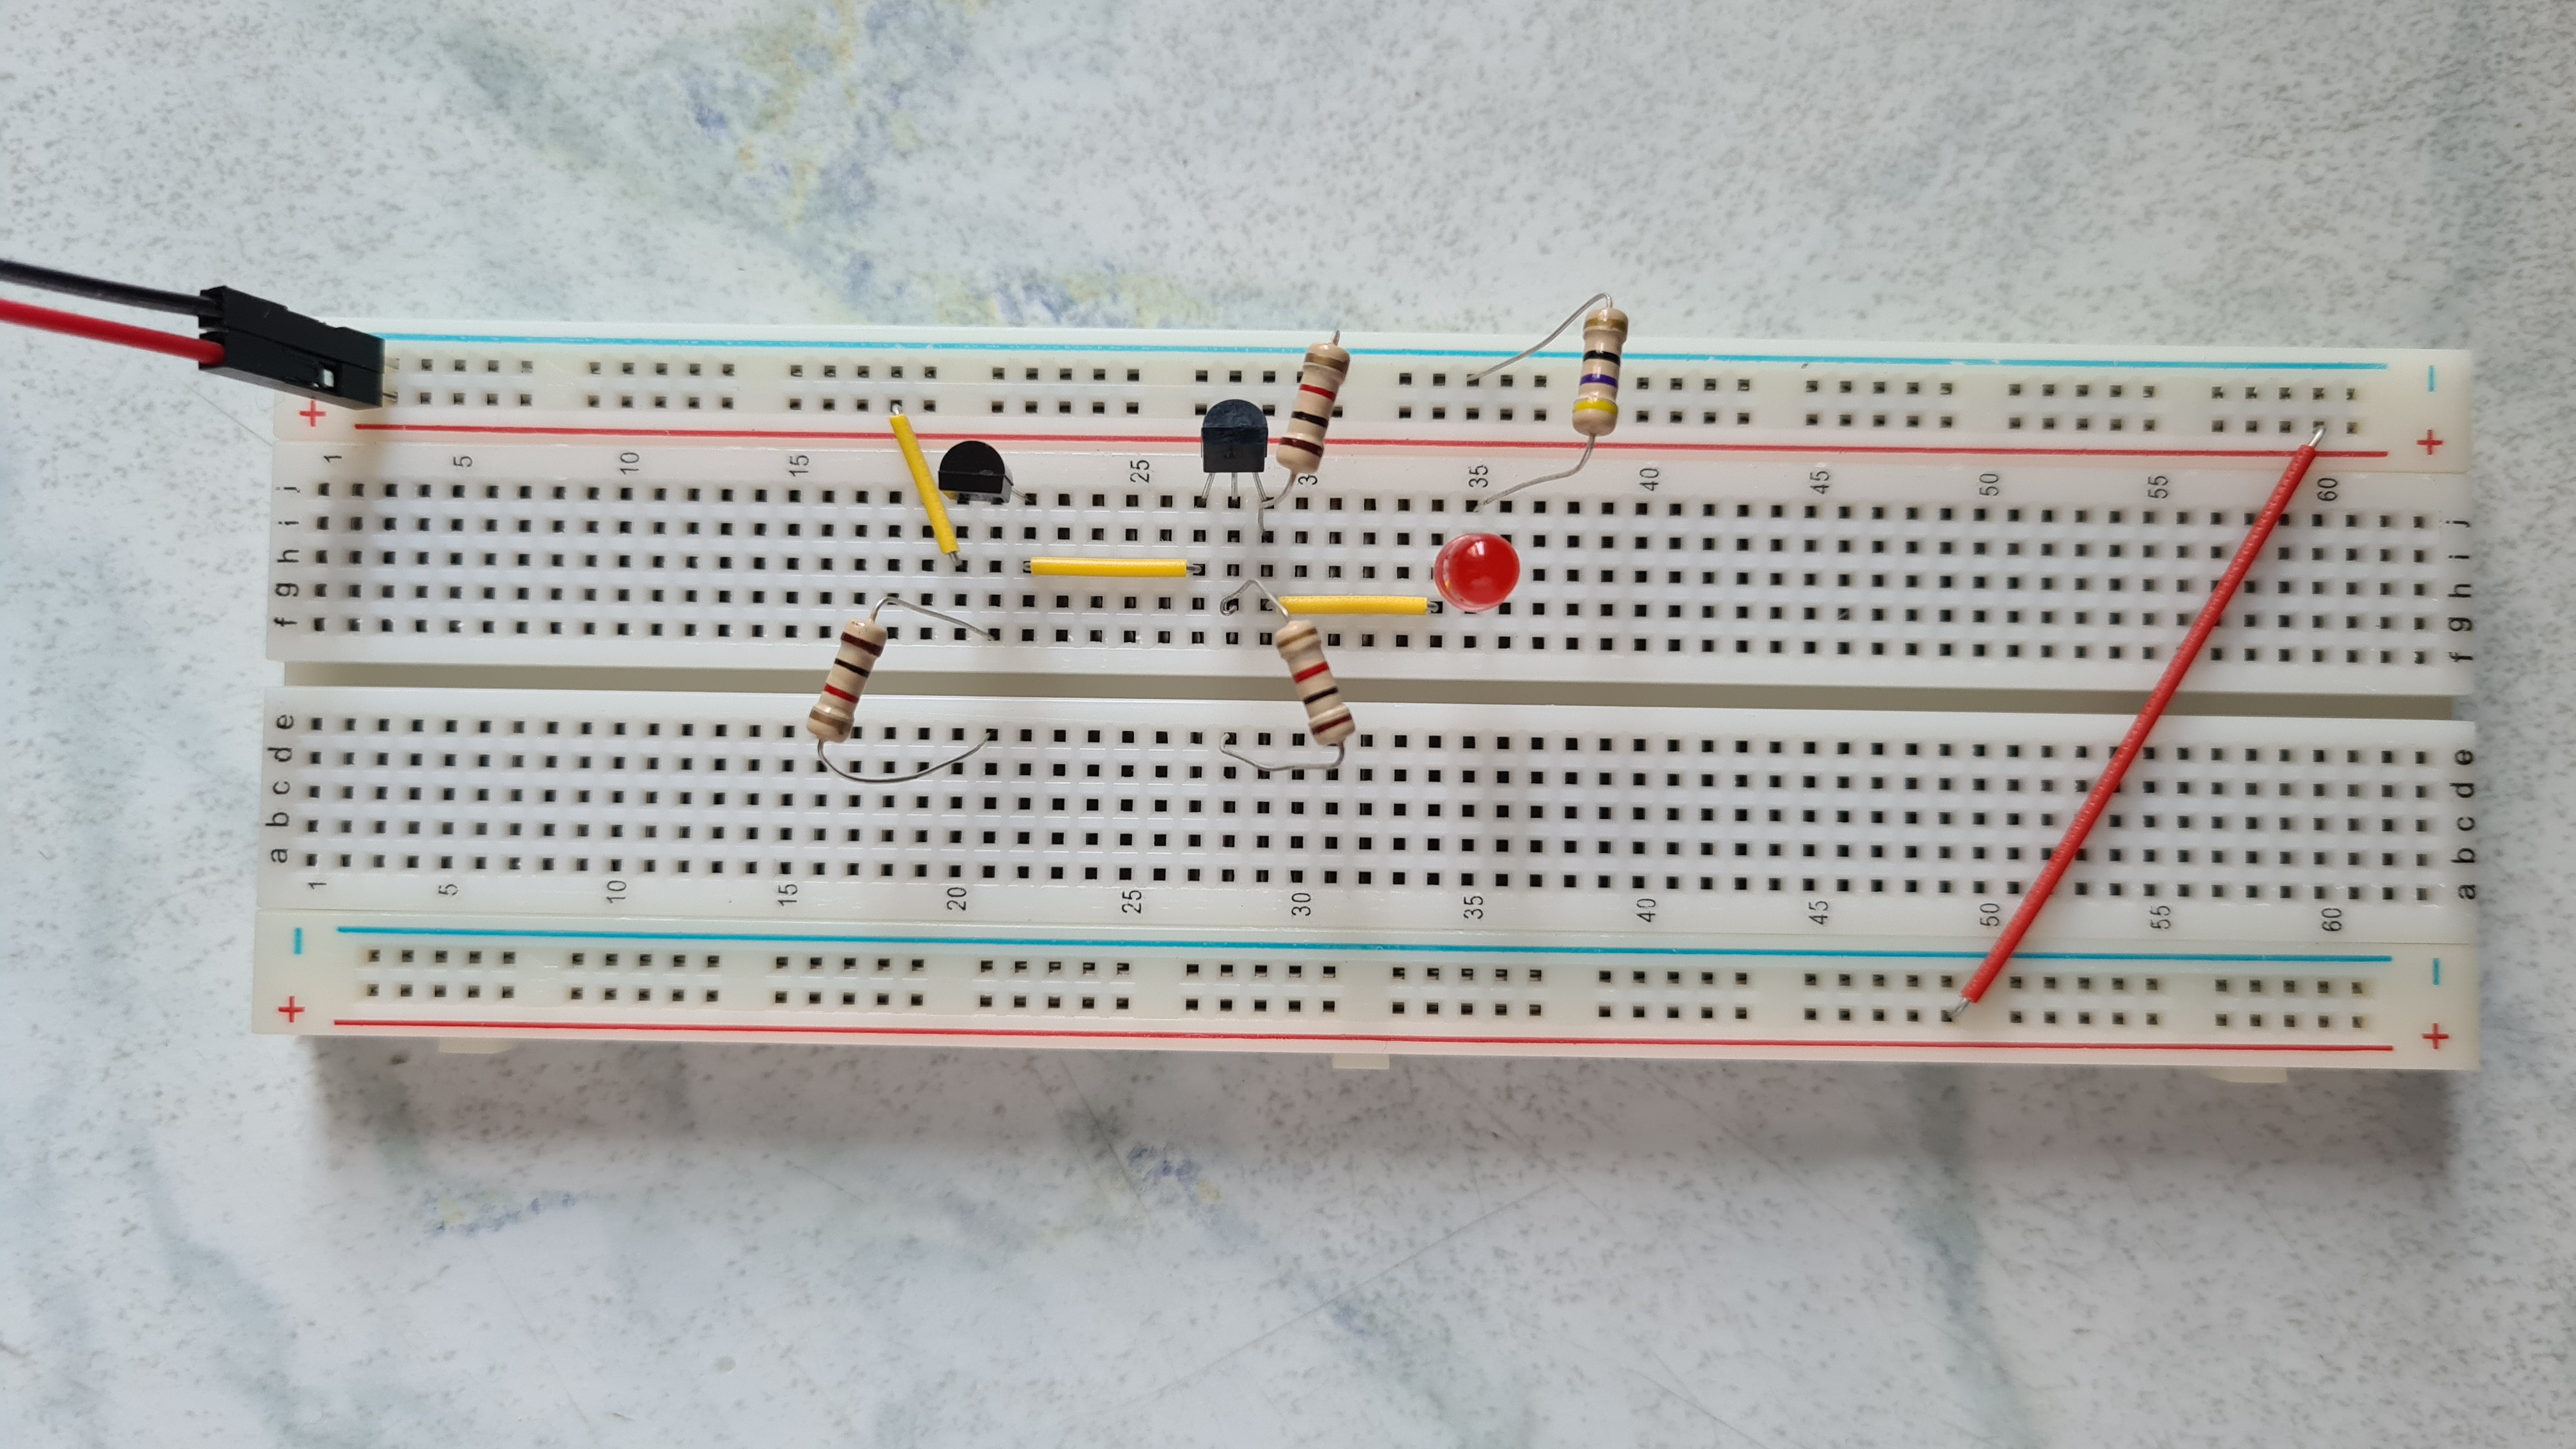
\includegraphics[height=4cm, keepaspectratio]{./Fotos/UND-00.jpg}
		\vspace{1cm}
	\end{minipage}%
	\begin{minipage}{.5\textwidth}
		\centering
		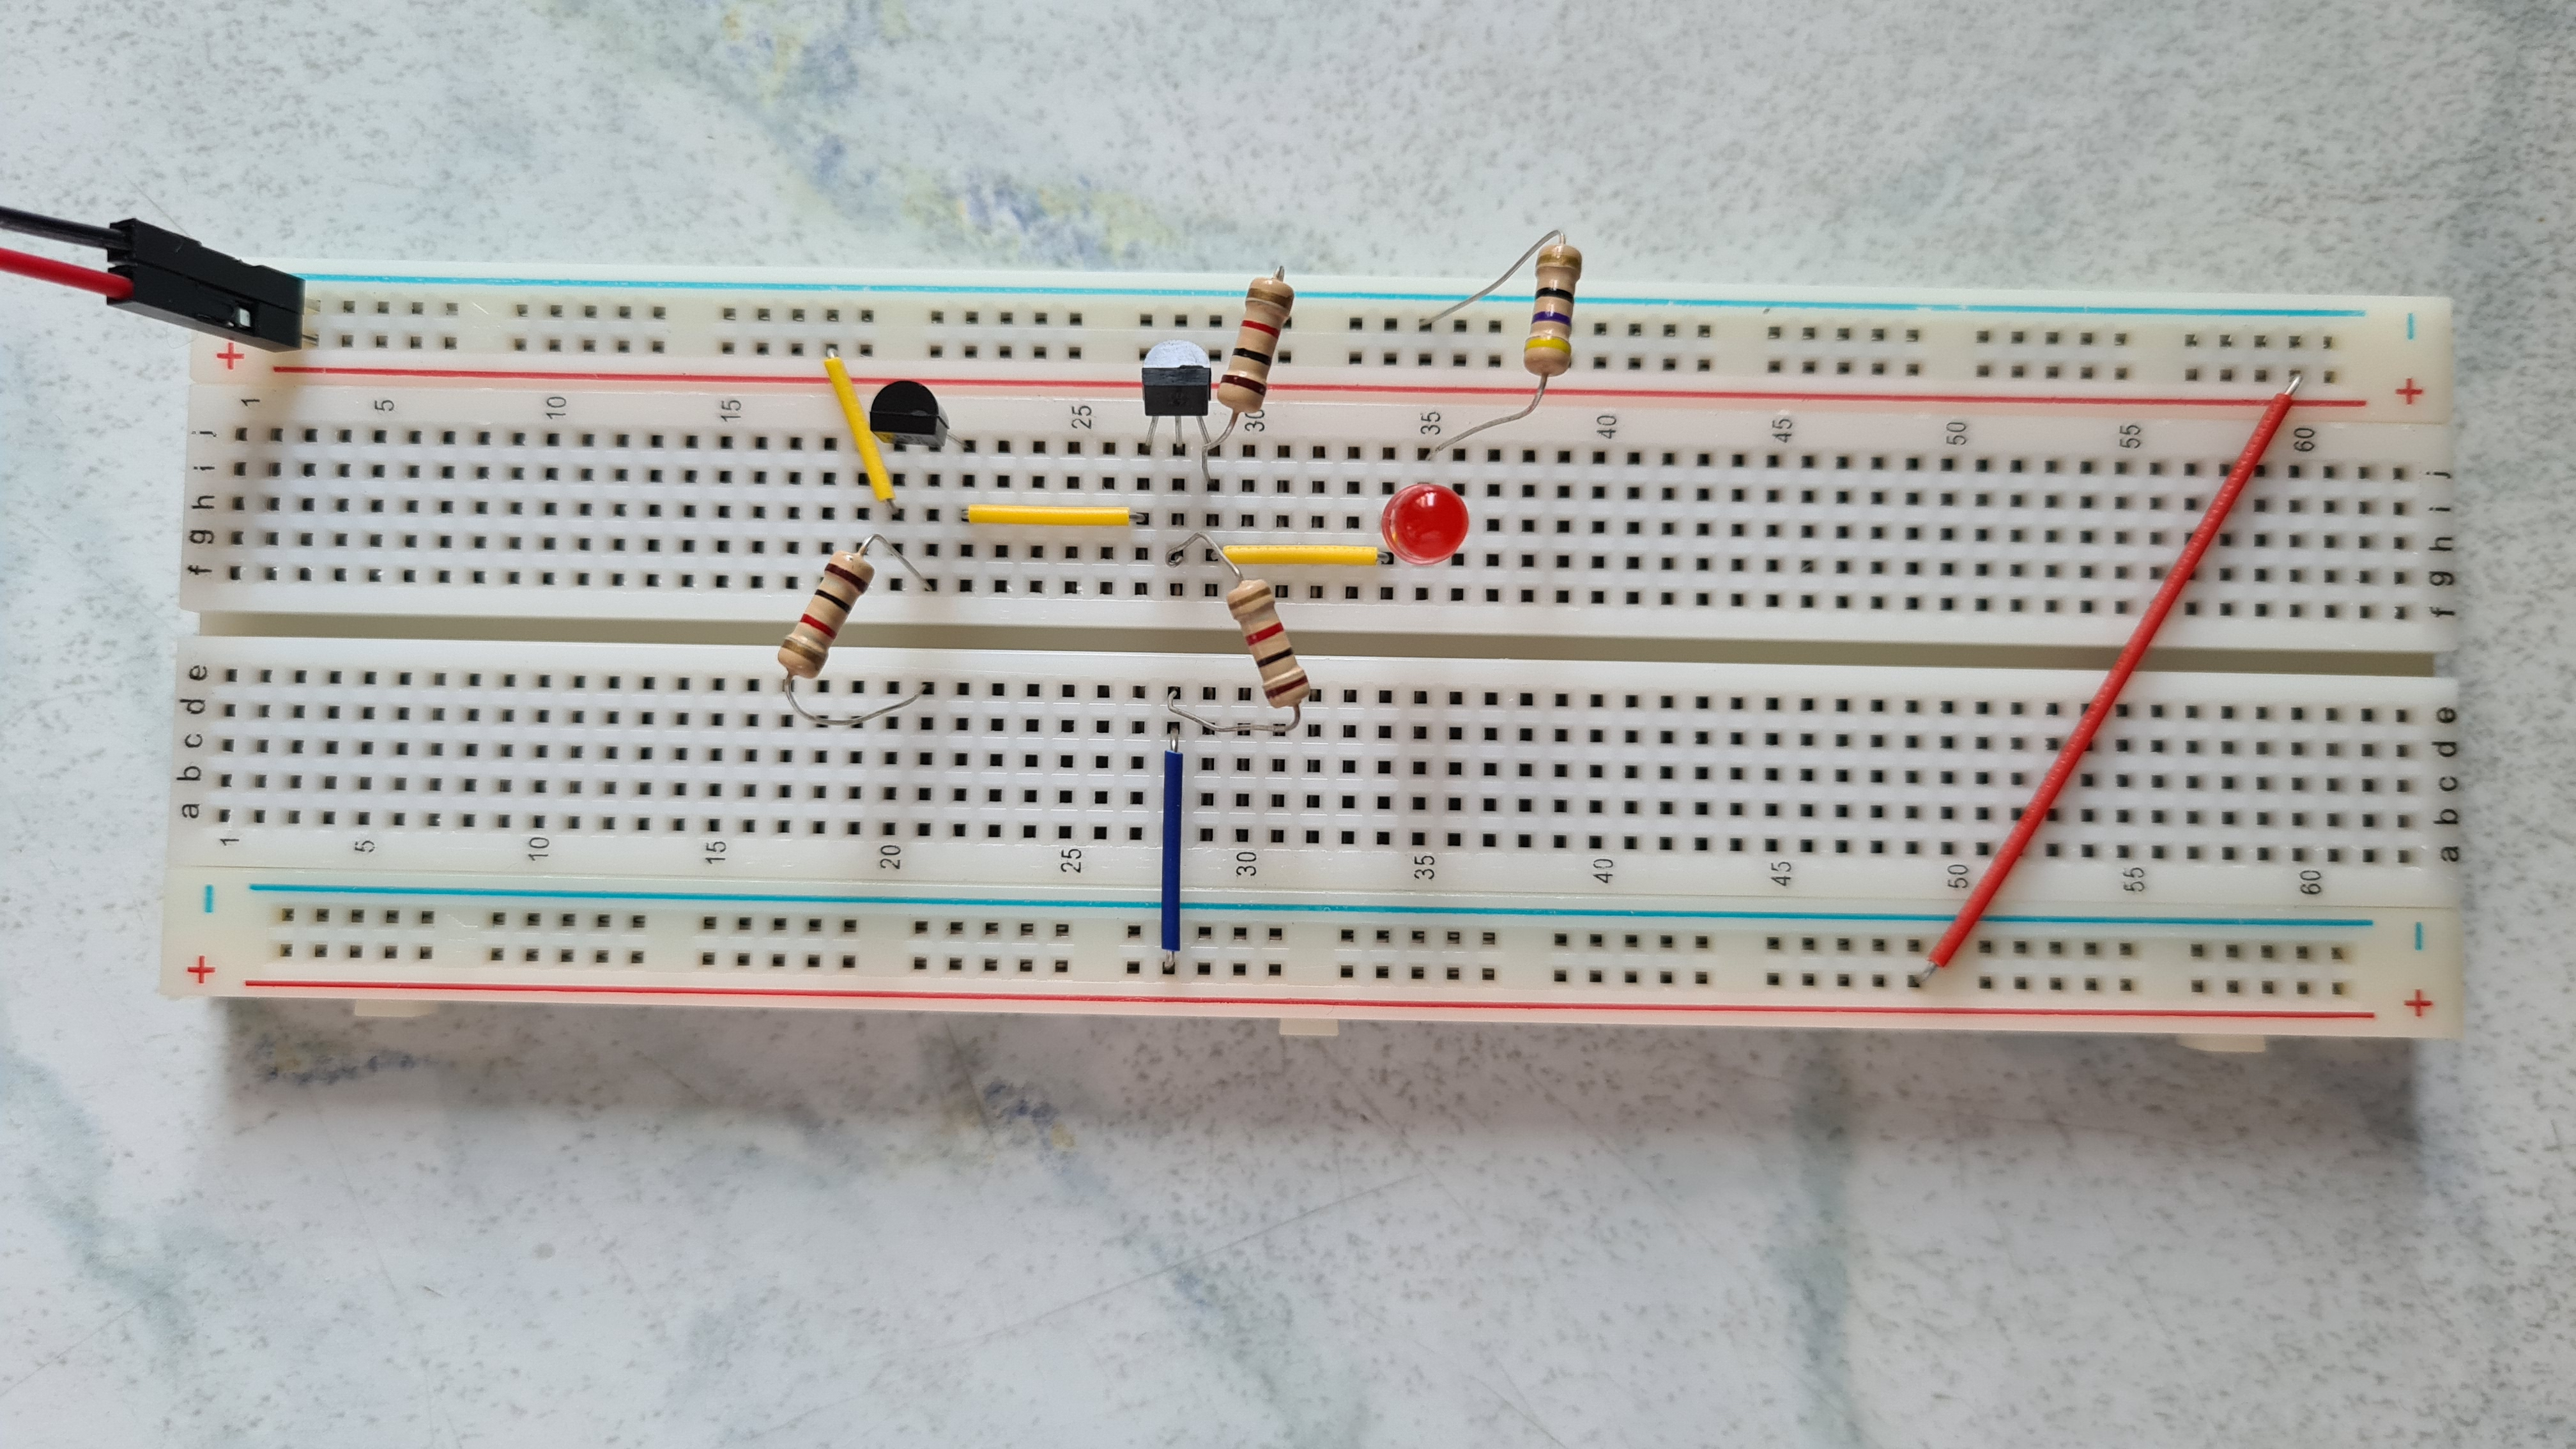
\includegraphics[height=4cm, keepaspectratio]{./Fotos/UND-01.jpg}
		\vspace{1cm}
	\end{minipage}
	\begin{minipage}{.5\textwidth}
		\centering
		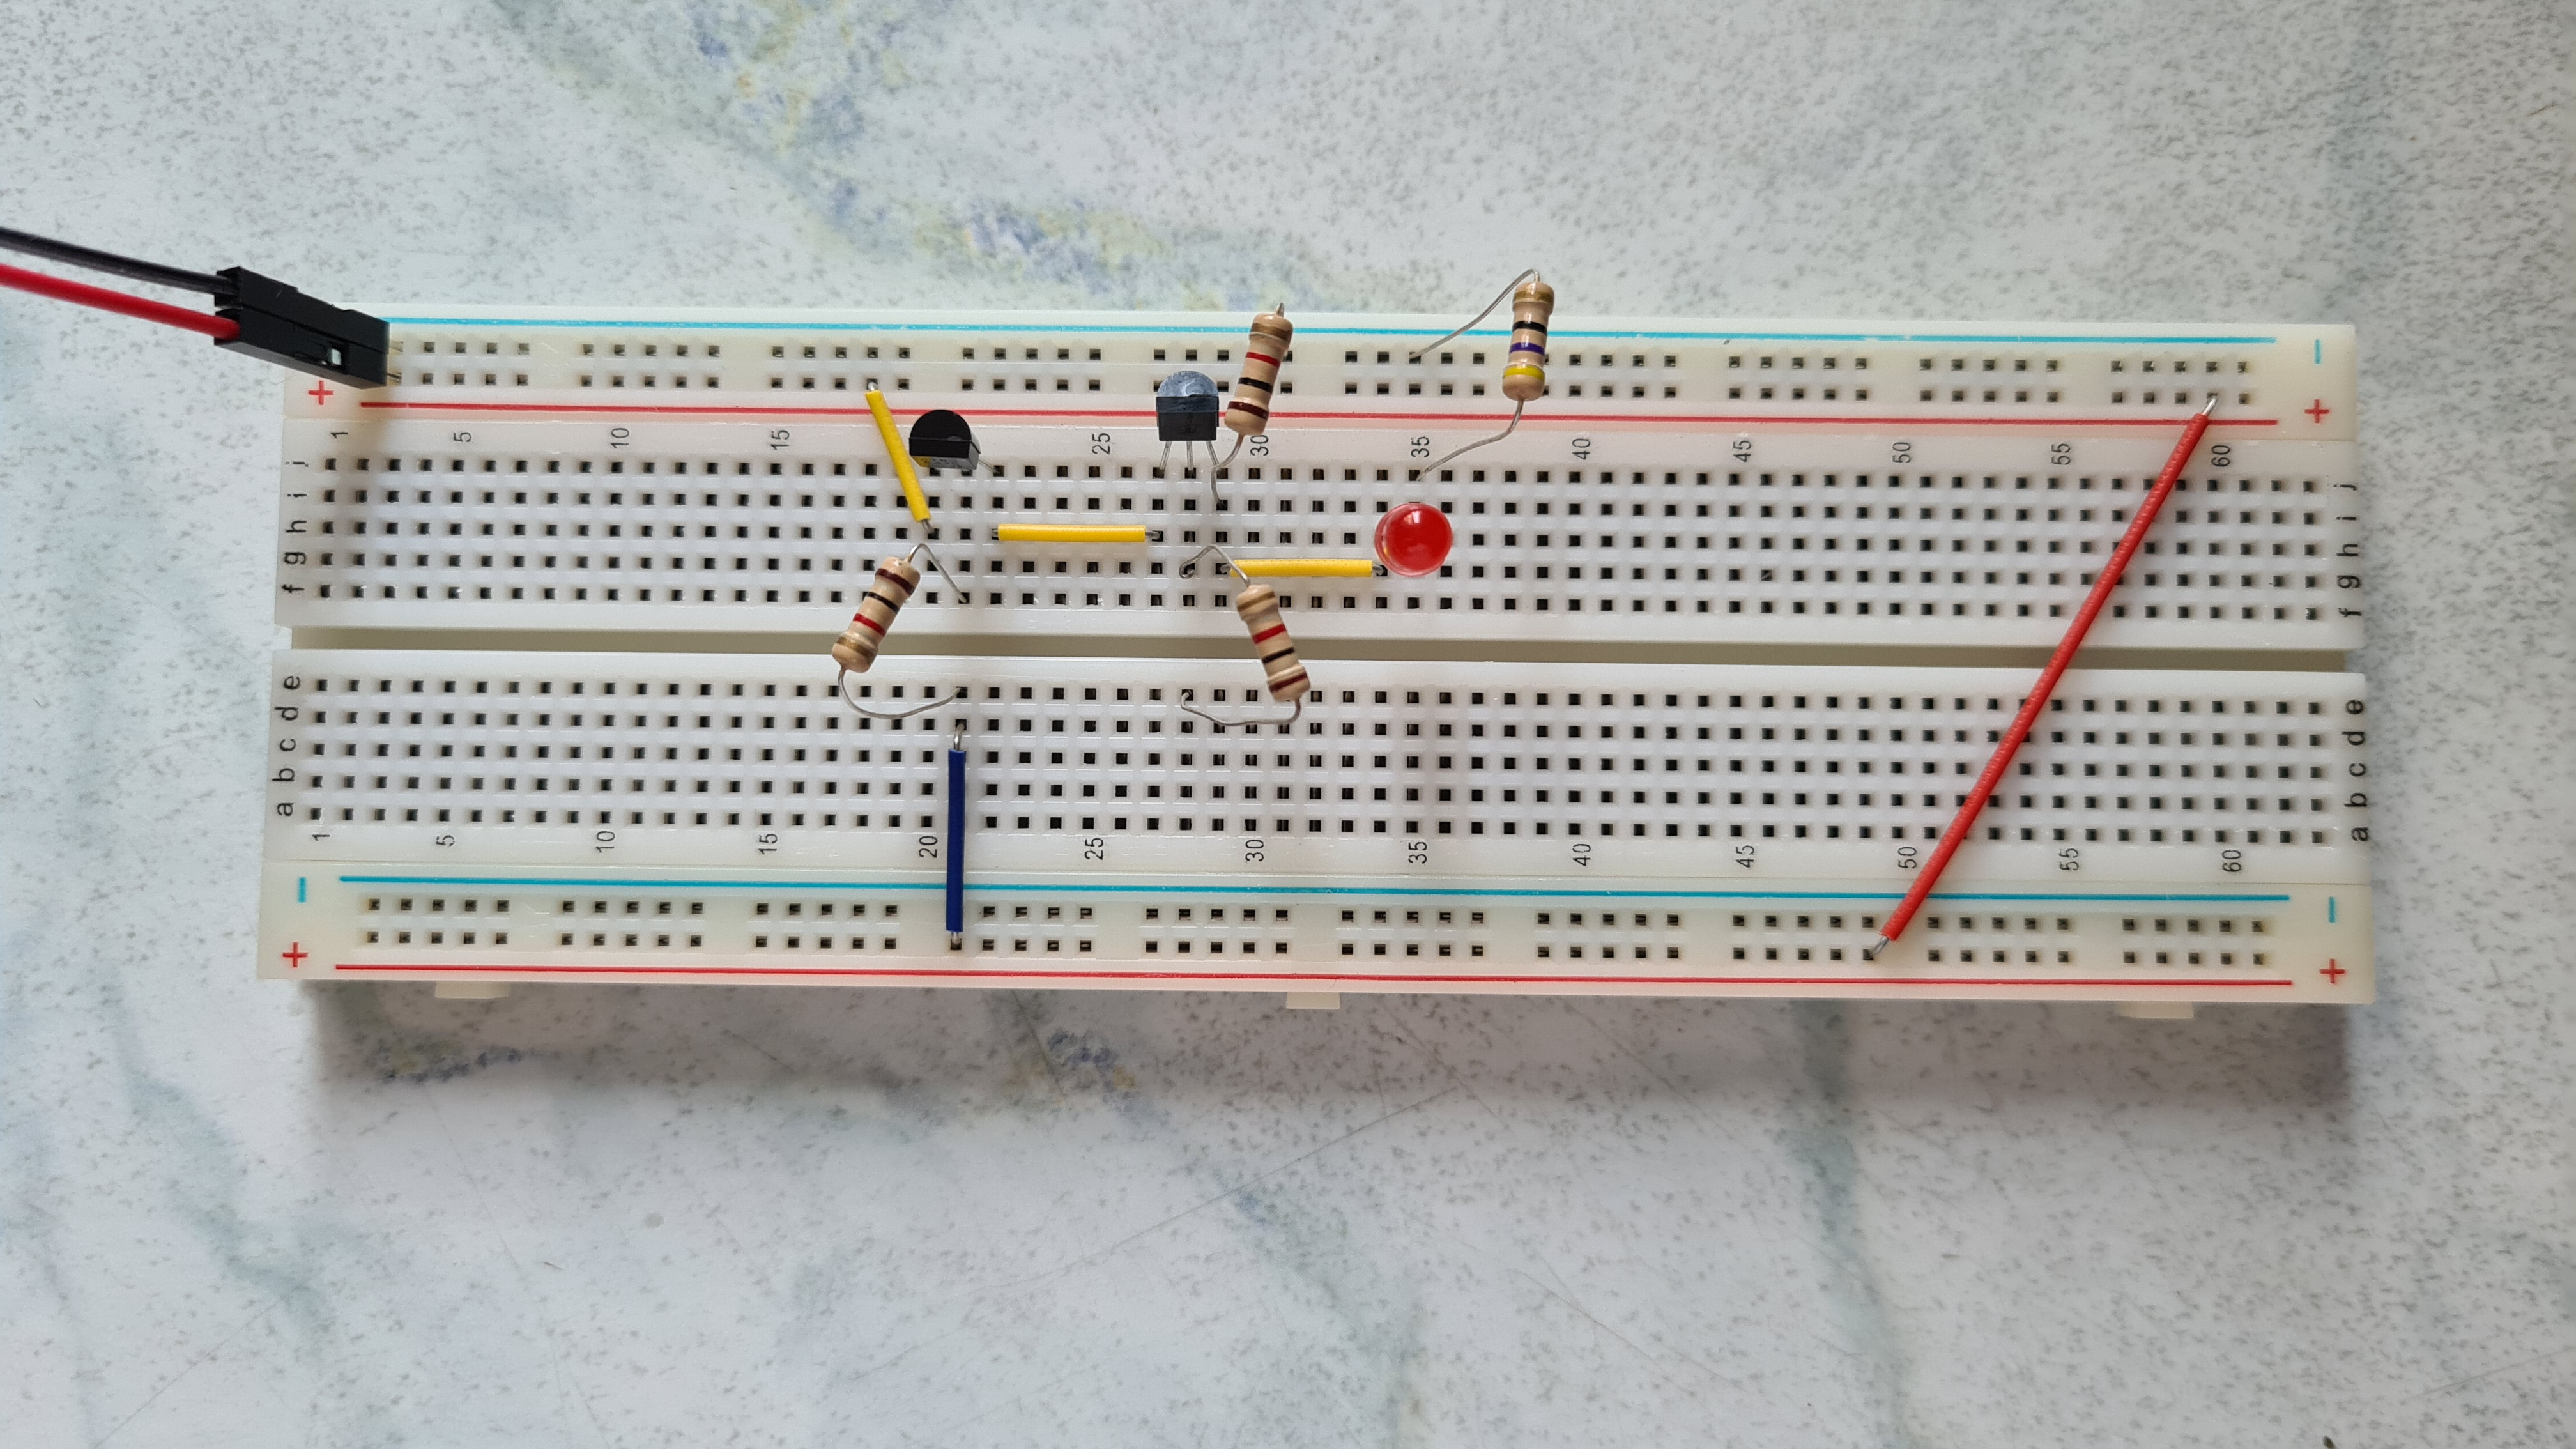
\includegraphics[height=4cm, keepaspectratio]{./Fotos/UND-10.jpg}
	\end{minipage}%
	\begin{minipage}{.5\textwidth}
		\centering
		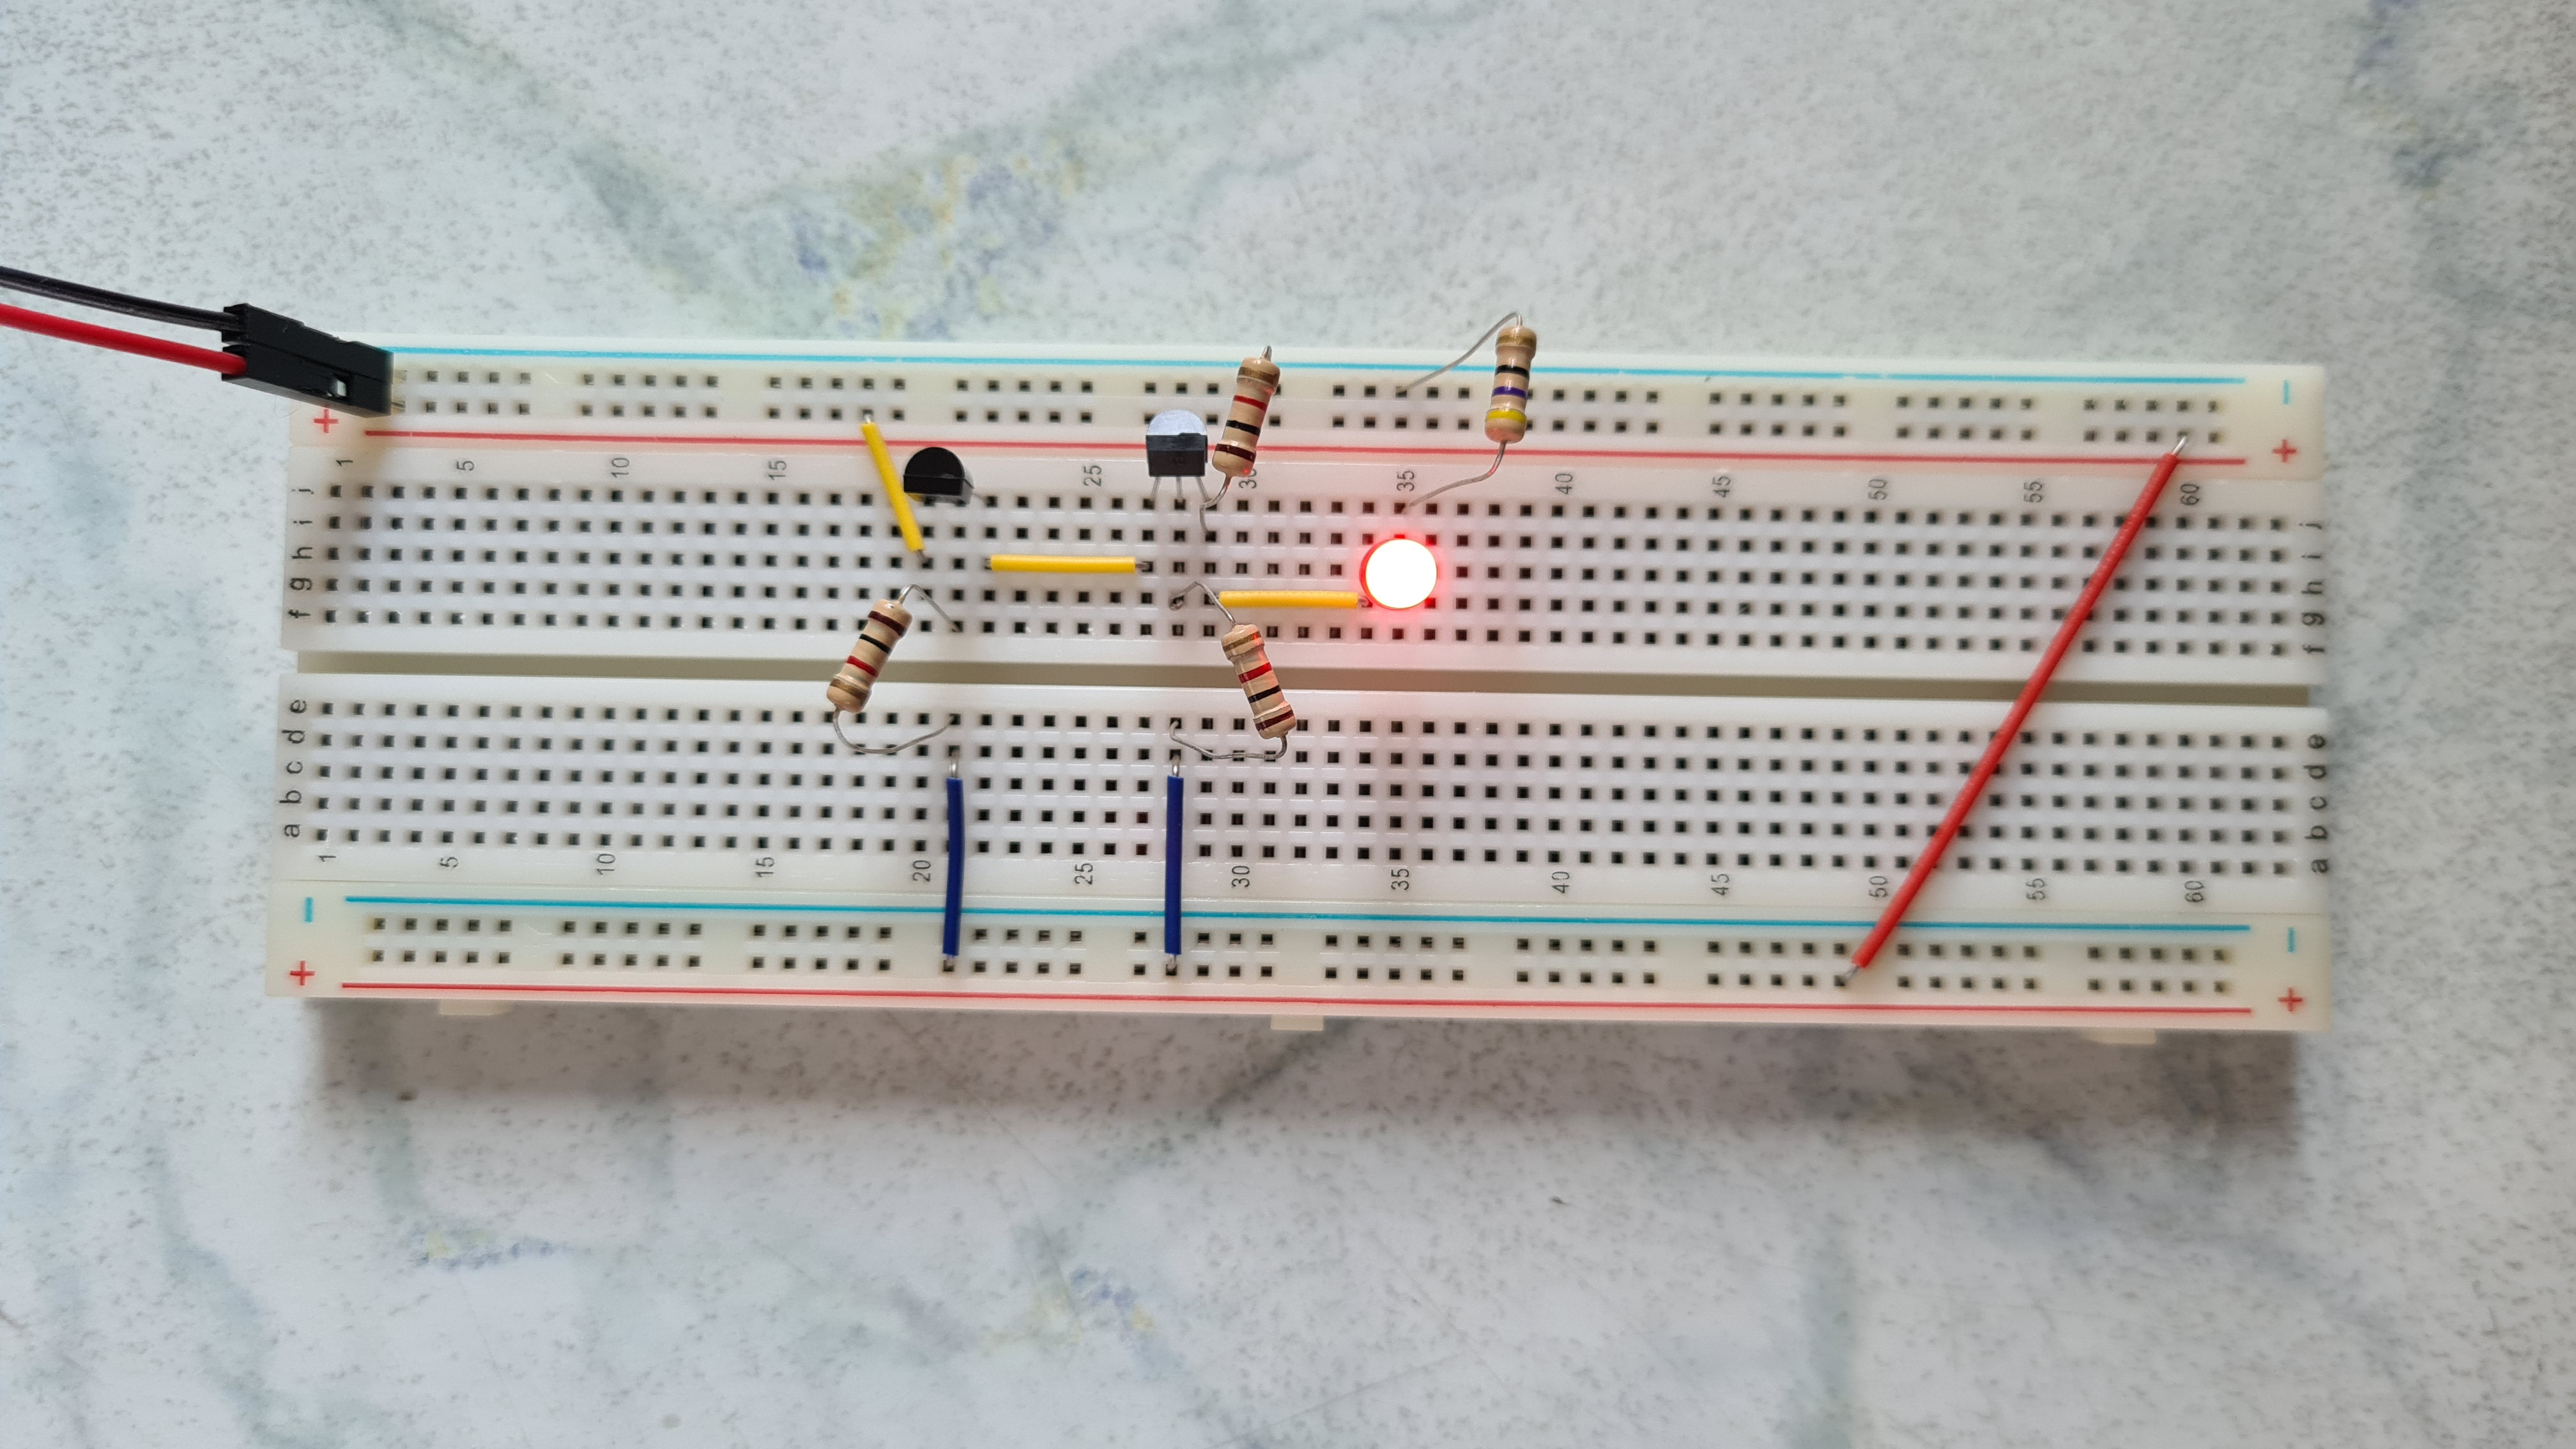
\includegraphics[height=4cm, keepaspectratio]{./Fotos/UND-11.jpg}
	\end{minipage}
	\caption{Praktischer Aufbau des UND-Gatters in allen möglichen Zuständen.}
\end{figure}
\newpage
Diese Abbildung zeigt das logische UND-Gatter auf einem Steckbrett. Die vier möglichen Zustände der Eingabeanschlüsse sind durch die blauen Drähte gegen \glqq{}+\grqq{} erkennbar. Im letzten Bild sind A und B durch diese Drähte mit HIGH verbunden. Die dadurch anliegende Spannung an Out ist durch die leuchtende LED zu erkennen.

\subsection{ODER-Gatter}
\begin{figure}[h]
	\centering
	\hspace{1cm}
	\begin{tabular}{|c|c|c|}
		\hline
		\textbf{A} & \textbf{B} & \textbf{Out} \\
		\hline
		0 & 0 & 0 \\
		1 & 0 & 1 \\
		0 & 1 & 1 \\
		1 & 1 & 1 \\
		\hline
	\end{tabular}
	\caption{Wahrheitstabelle für das logische ODER-Gatter}
\end{figure}
Der Aufbau des ODER-Gatters ist dem des UND-Gatters ähnlich. Die Wahrheitstabelle zeigt, das hier Out auf HIGH liegt, sobald entweder A oder B auf HIGH liegen.
\newpage
\begin{figure}[h!]
	\centering
	\begin{circuitikz}
		\draw (0, 0) node[npn](T1){$T_1$};
		\draw (2, -2) node[npn](T2){$T_2$};
		
		
		\draw (T1.B) to[R, l=$R_1$, a=\SI{1}{k\ohm}] ++(-2, 0) to[short, -o] ++(-.5, 0) node[left]{A};
		\draw (T2.B) to[R, l=$R_2$, a=\SI{1}{k\ohm}] ++(-4, 0) to[short, -o] ++(-.5, 0) node[left]{B};
		
		\draw (T1.C) to[short, -o] ++(0, 1) node[above]{$VCC$};
		\draw (T2.C) to[short] ++(0, 2) to[short, -*] ++(-2, 0);
		
		\draw (T1.E) to[short] ++(3, 0) to[short, -*] ++(0, -2);
		\draw (T2.E)++(1, 0) to[R, l=$R_3$, a=\SI{100}{\ohm}] ++(0, -2) to[short] ++(0, -.5) node[ground](GND){};
		
		\draw (T2.E) to[short, -o] ++(3, 0) node[right]{Out};
		
		\draw[gray, very thick, densely dashed] (-3, 3) -- (4.5, 3) -- (4.5, -6) -- (-3, -6) -- cycle;
		\draw (4.5, -6) node[above right, gray]{ODER-Gatter};
	\end{circuitikz}
	\caption{Schaltplan für die logische ODER-Schaltung mithilfe von npn-Transistoren.}
\end{figure}
Diese Abbildung beschreibt den Aufbau eines ODER-Gatters. Analog zum UND-Gatter liegen auch hier A und B jeweils an der Basis eines npn-Transistors. Die Kollektoren beider Transistoren sind hierbei mit VCC verbunden. Die Emitter der beiden von $T_1$ und $T_2$ sind beide mit Out verbunden. Auch hier liegt an Out ein Widerstand gegen das Nullpotenzial an. Falls A und B auf LOW gesetzt sind, ist Out ebenso auf LOW. 
\begin{figure}[h!]
	\begin{minipage}{.5\textwidth}
		\centering
		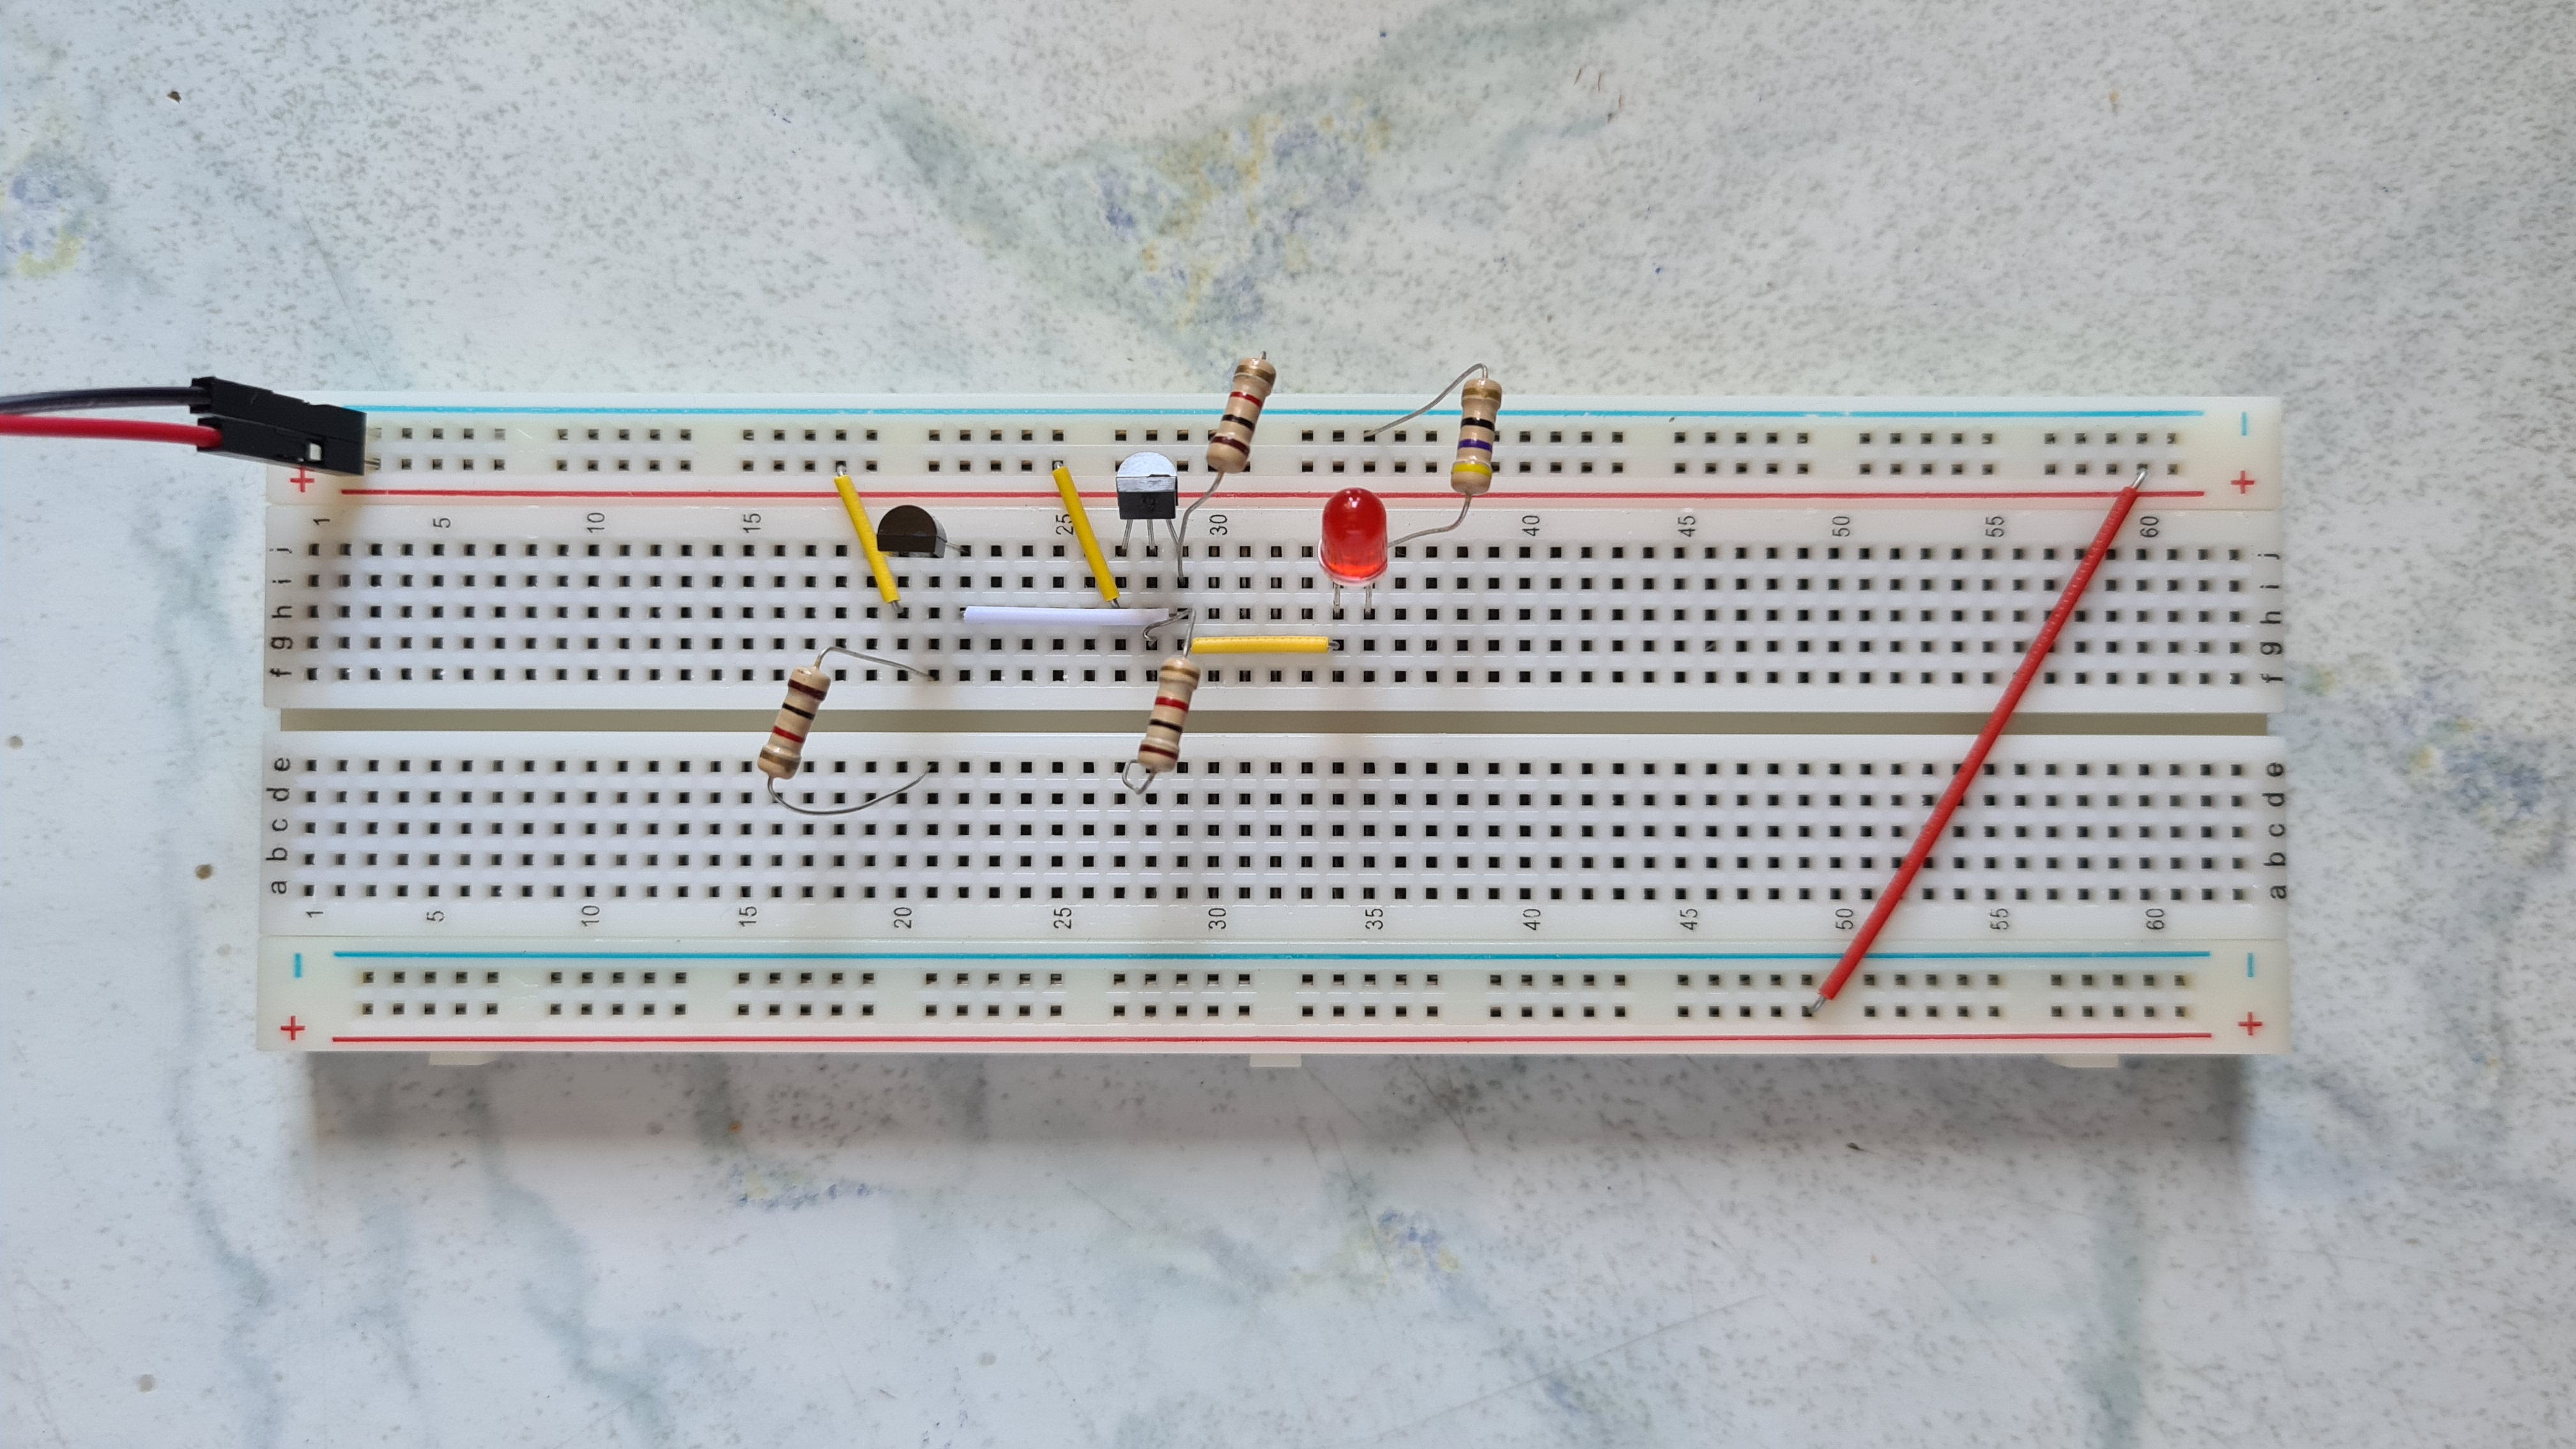
\includegraphics[height=4cm, keepaspectratio]{./Fotos/ODER-00.jpg}
		\vspace{1cm}
	\end{minipage}%
	\begin{minipage}{.5\textwidth}
		\centering
		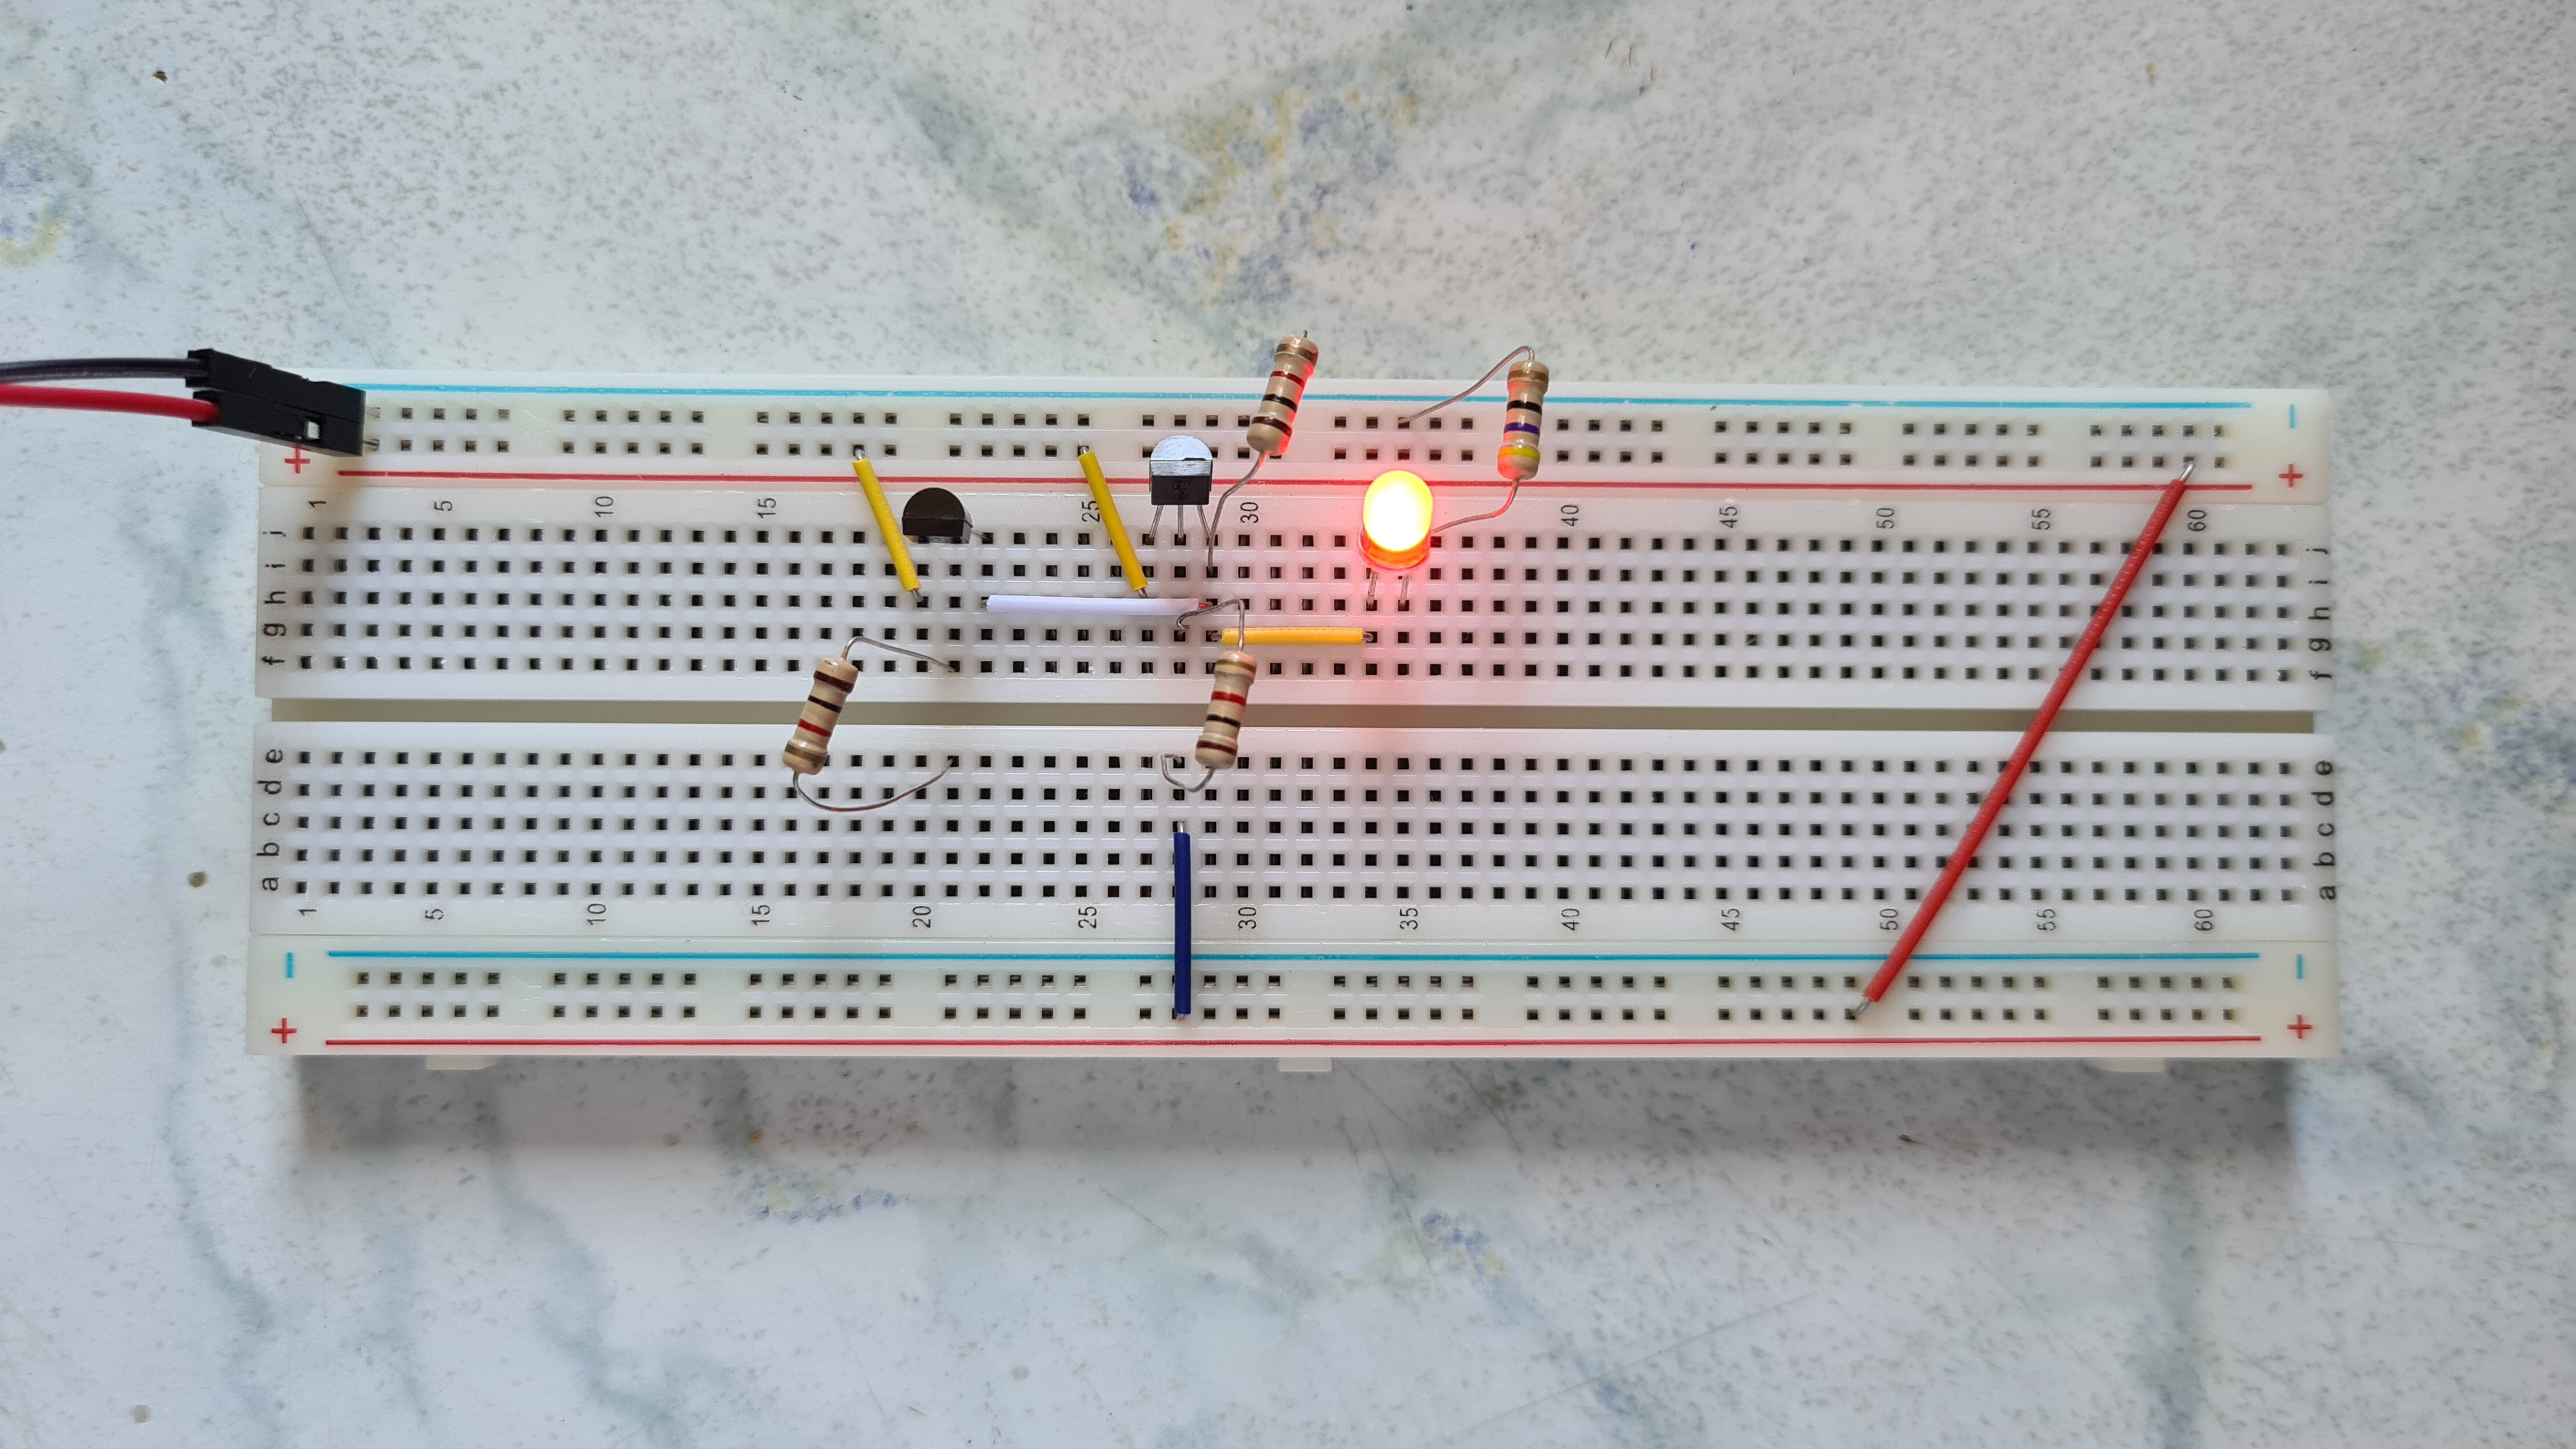
\includegraphics[height=4cm, keepaspectratio]{./Fotos/ODER-01.jpg}
		\vspace{1cm}
	\end{minipage}
	\begin{minipage}{.5\textwidth}
		\centering
		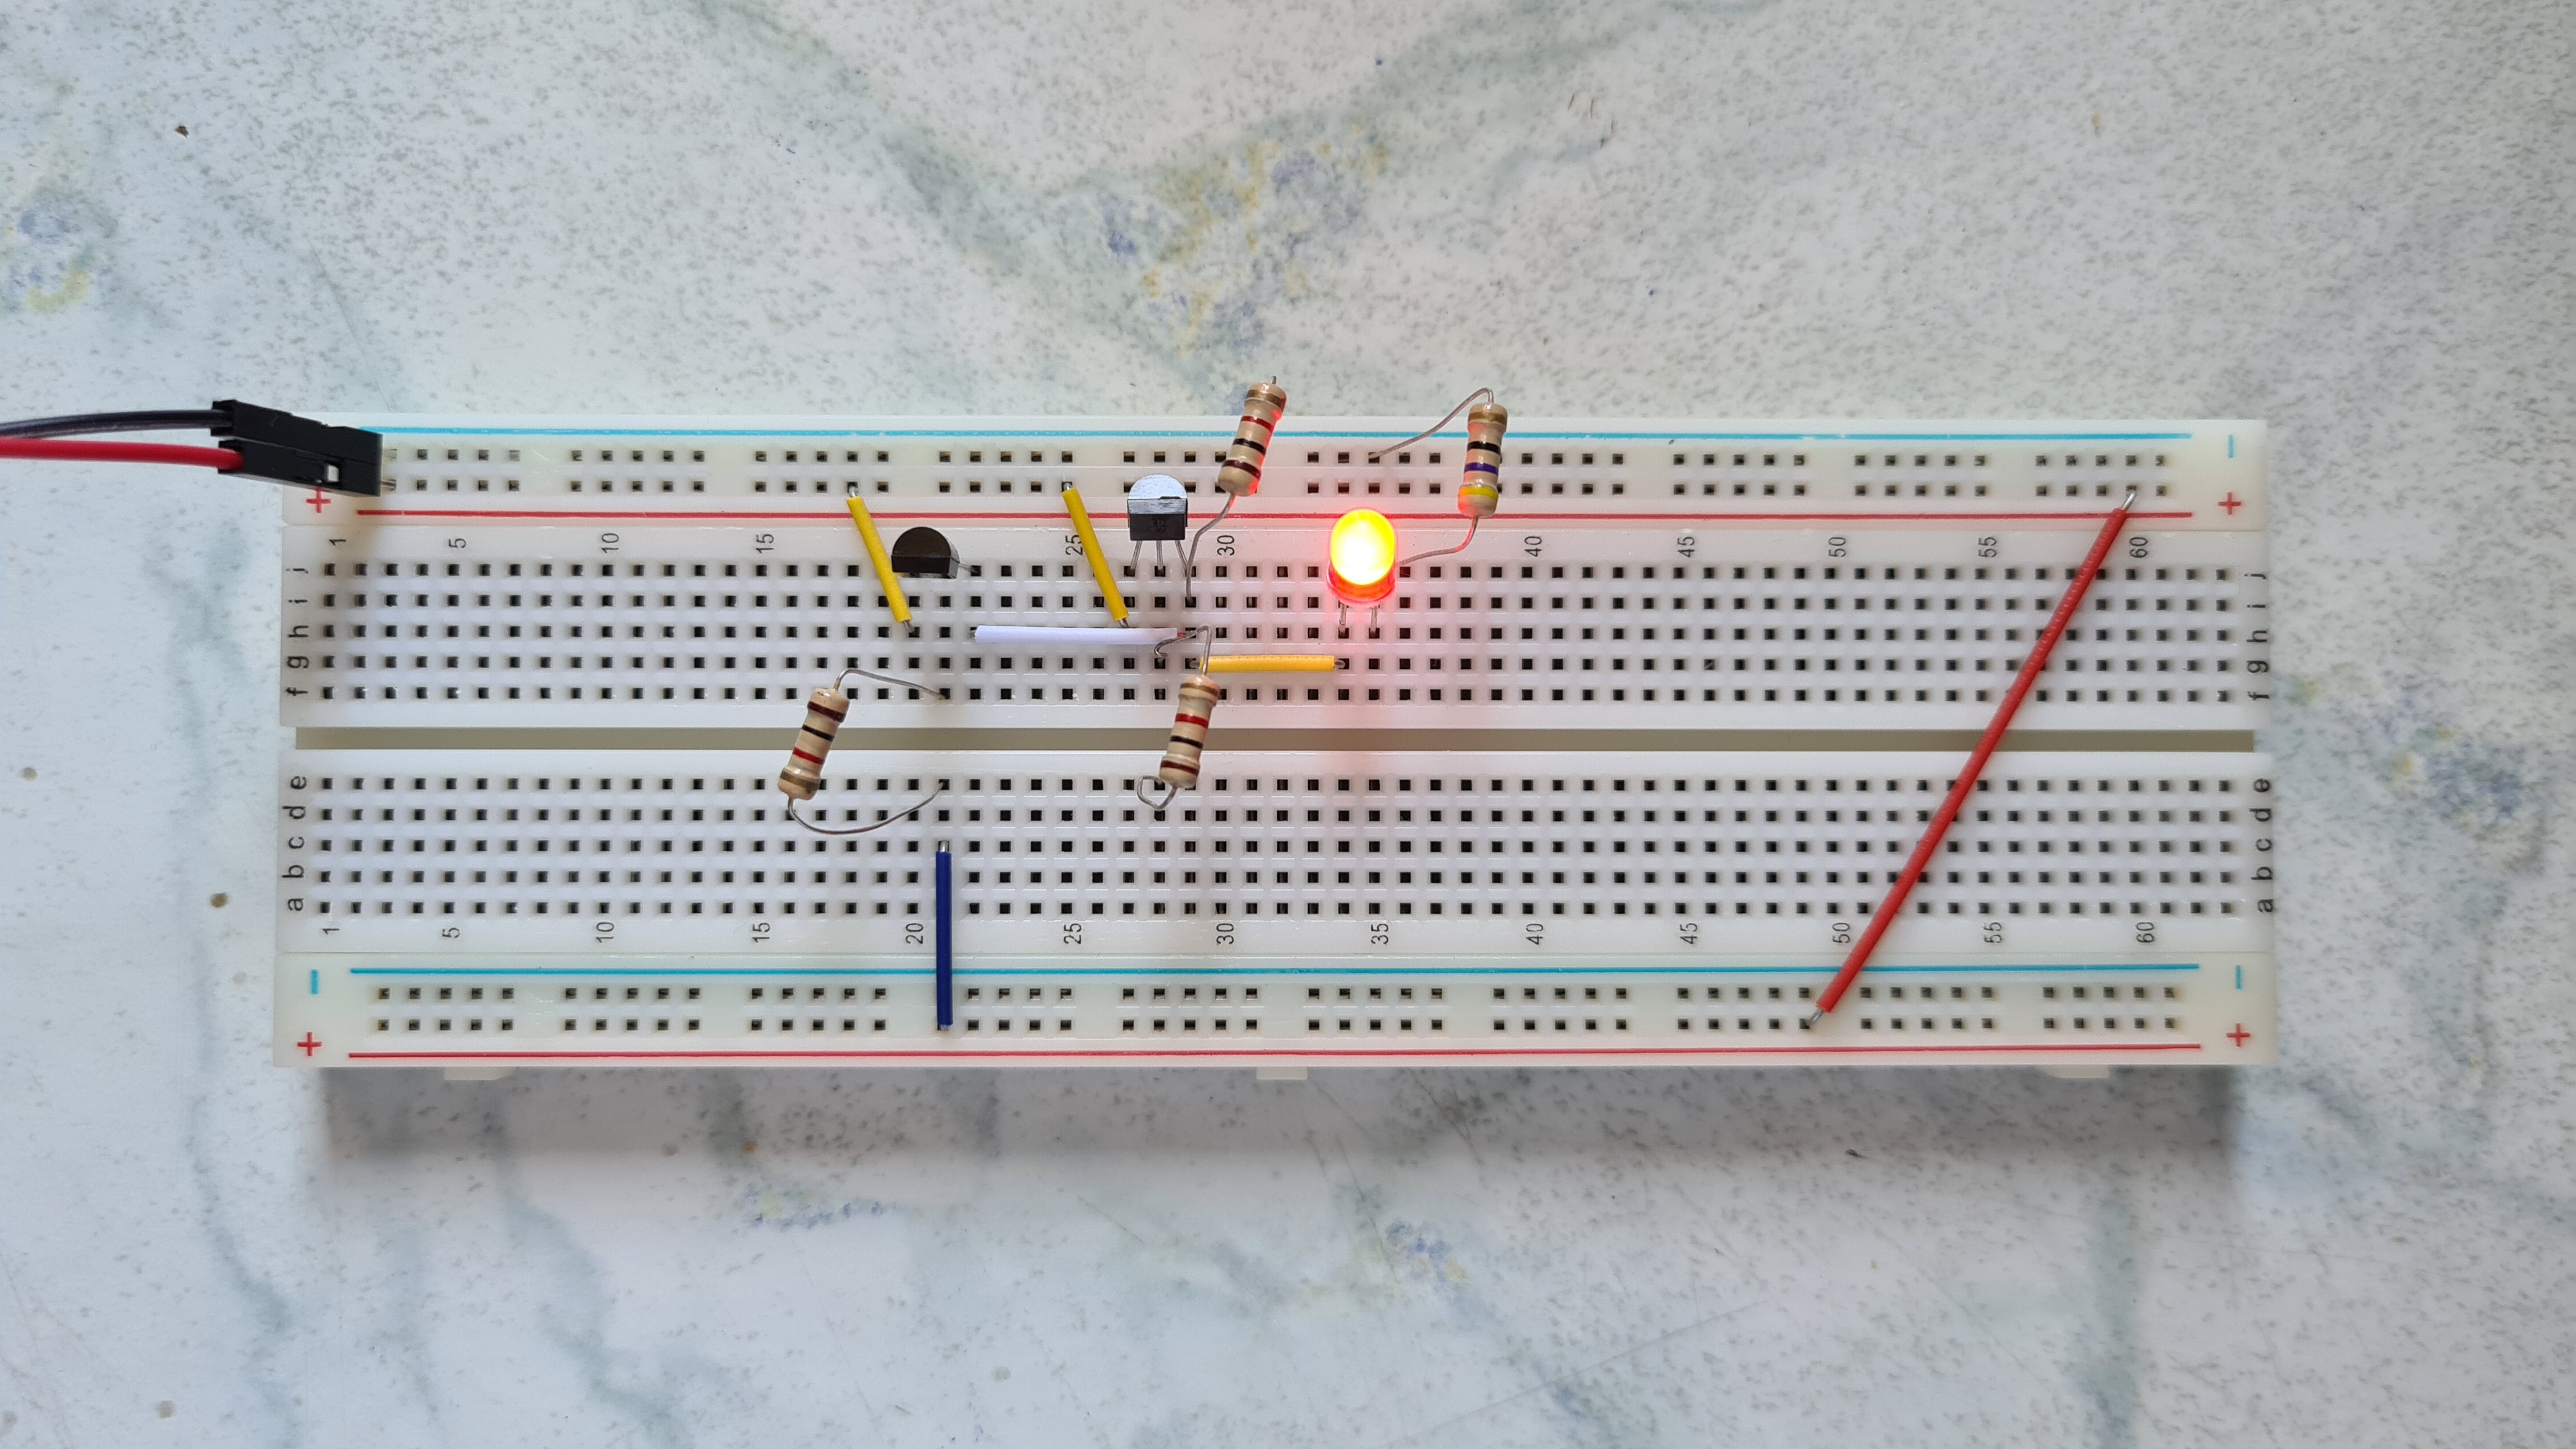
\includegraphics[height=4cm, keepaspectratio]{./Fotos/ODER-10.jpg}
	\end{minipage}%
	\begin{minipage}{.5\textwidth}
		\centering
		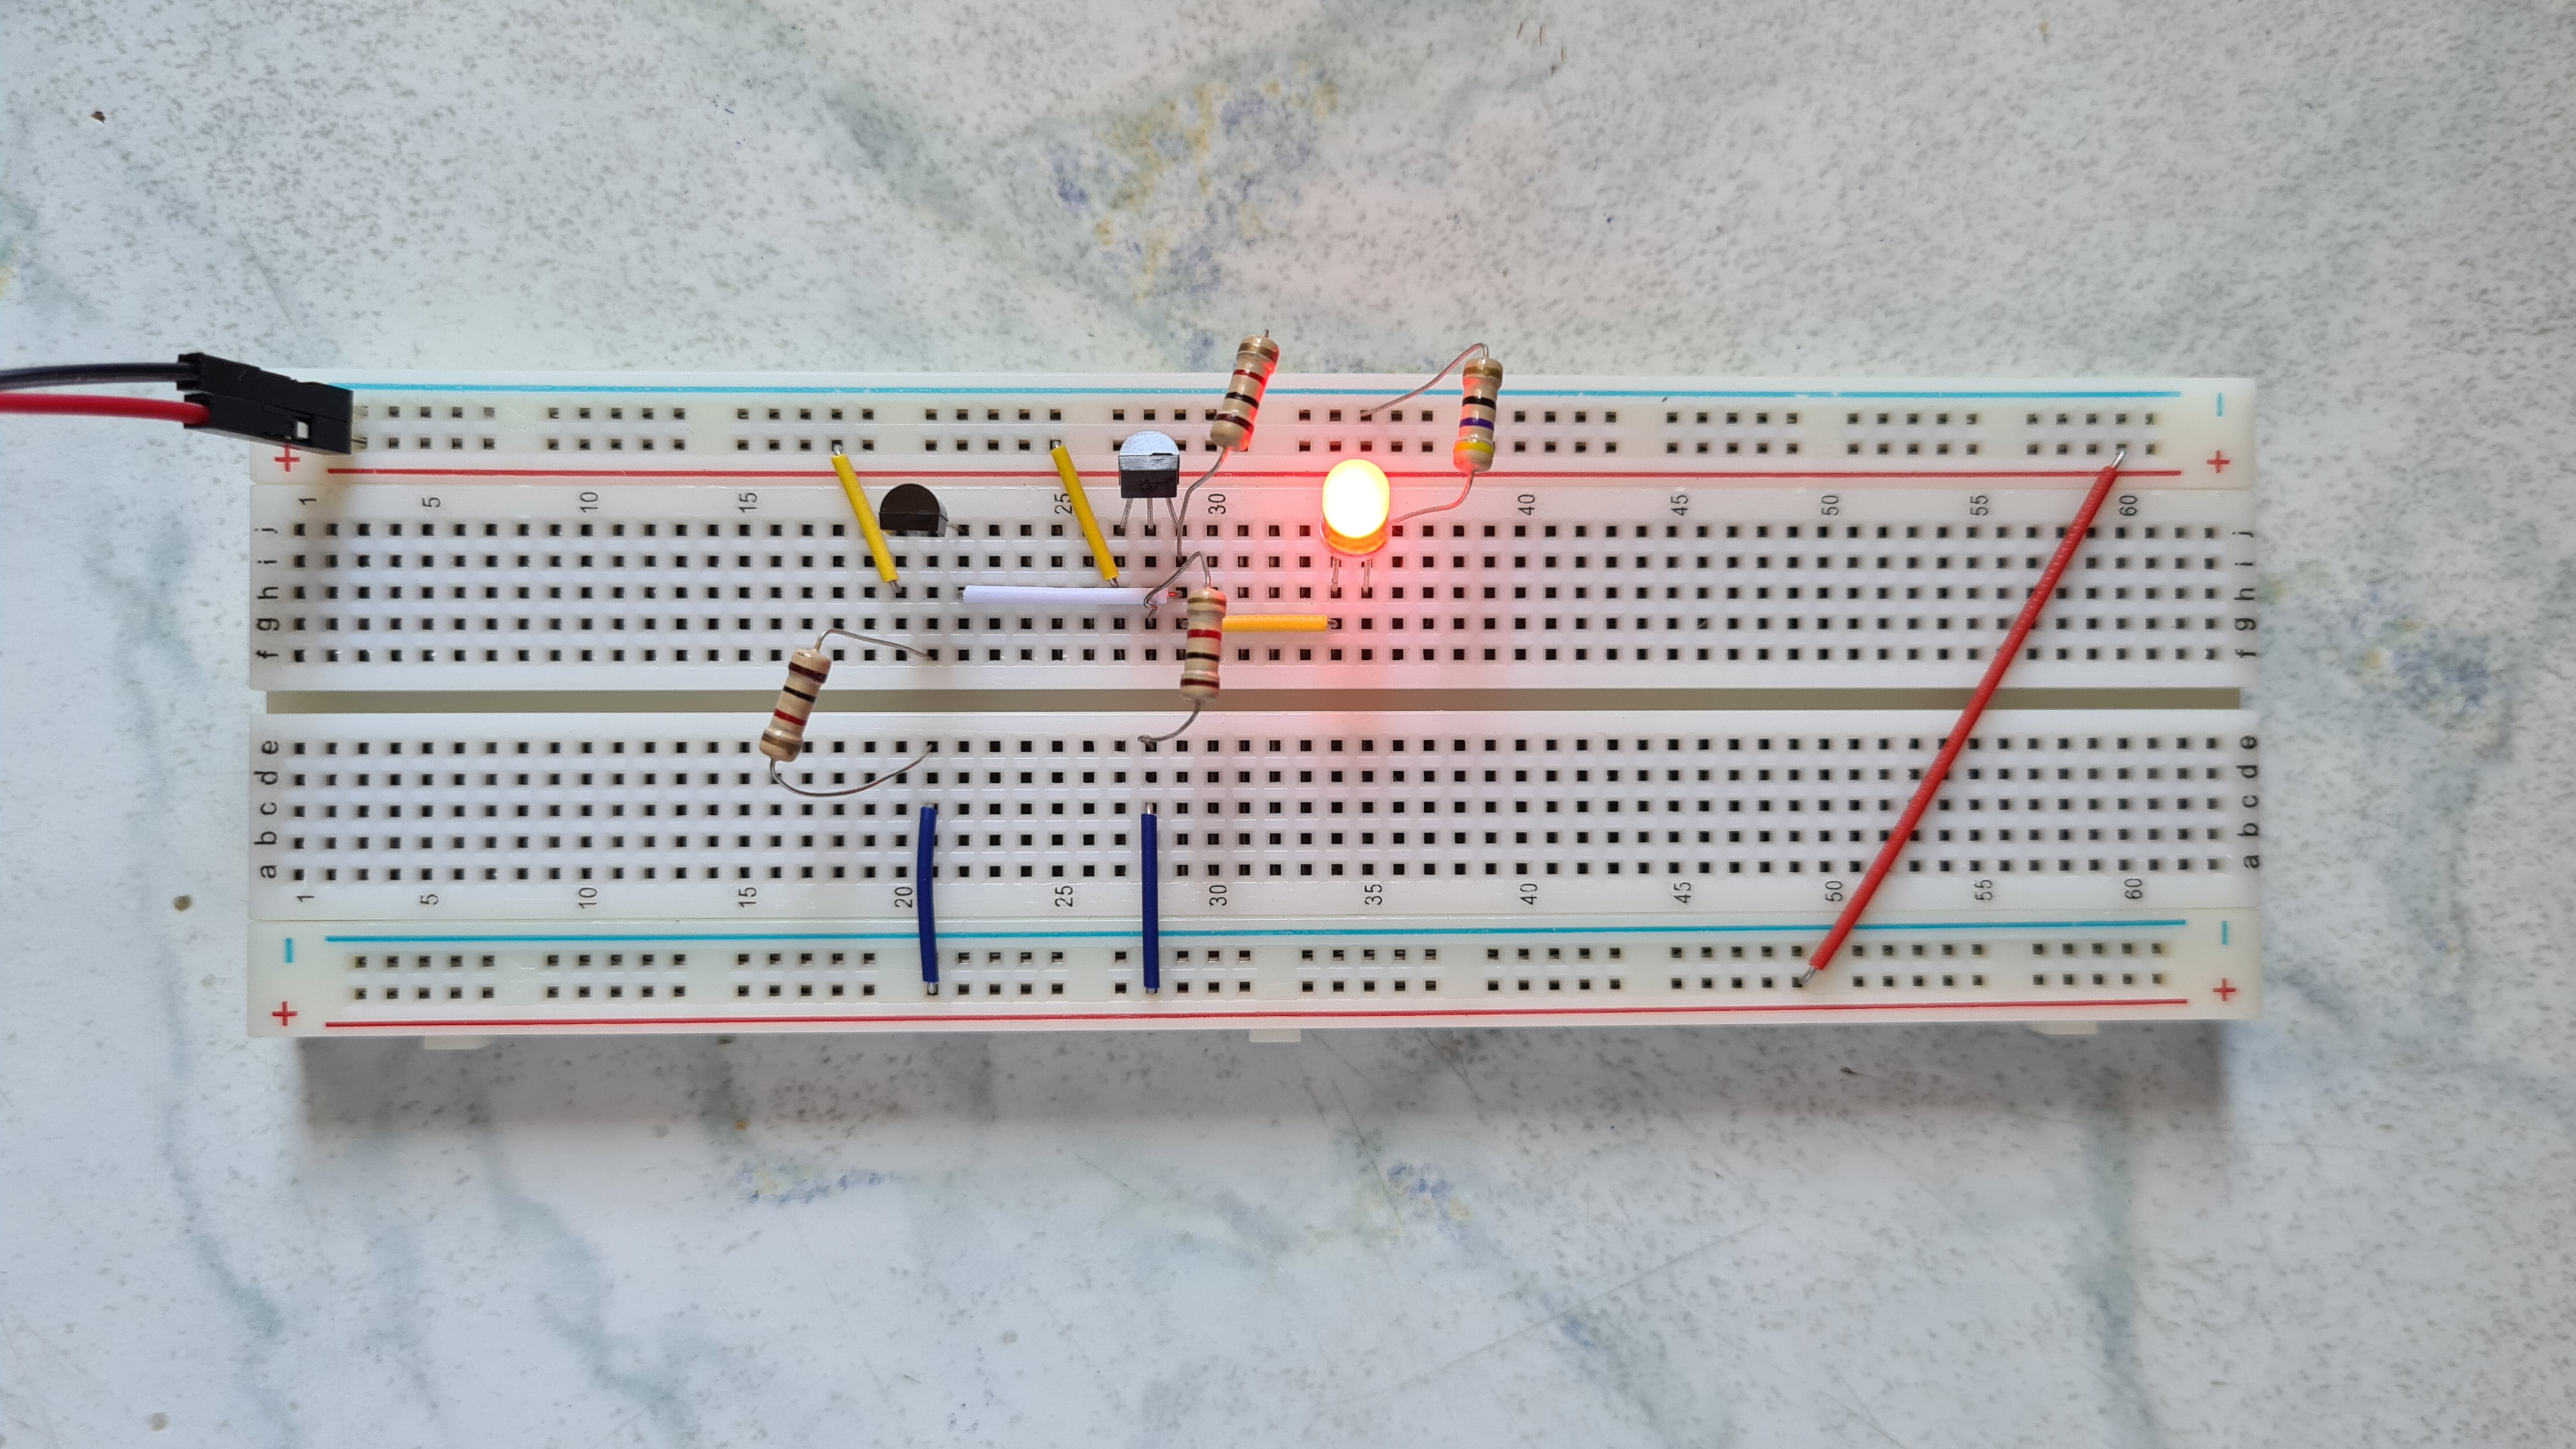
\includegraphics[height=4cm, keepaspectratio]{./Fotos/ODER-11.jpg}
	\end{minipage}
	\caption{Praktischer Aufbau des ODER-Gatters in allen möglichen Zuständen.}
\end{figure}
\newpage

\subsection{NICHT-Gatter}
\begin{figure}[h]
	\centering
	\hspace{1cm}
	\begin{tabular}{|c|c|}
		\hline
		\textbf{In} & \textbf{Out} \\
		\hline
		0 & 1 \\
		1 & 0 \\
		\hline
	\end{tabular}
	\caption{Wahrheitstabelle für das logische NICHT-Gatter}
\end{figure}
Das NICHT-Gatter besitzt lediglich einen Eingabeanschluss. Daher kann dieser auch als \glqq{}In\grqq{} bezeichnet werden. Out zeigt hier den gegenteiligen Zustand von In. So liegt Out beispielsweise auf HIGH, wenn In auf LOW gesetzt ist.\\
\begin{figure}[h!]
	\centering
	\begin{circuitikz}
		\draw (0, 0) node[npn](T1){$T_1$};
		
		\draw (T1.B) to[R, l=$R_1$, a=\SI{1}{k\ohm}] ++(-2, 0) to[short, -o] ++(-.5, 0) node[left]{In};
		
		\draw (T1.C) to[short] ++(0, .5) to[R, l=$R_2$, a=\SI{1}{k\ohm}, -o] ++(0, 2) node[above]{$VCC$};
		
		\draw (T1.E) to[short] (0, -1) node[ground](GND){};
		\draw (0, .75) to[short, *-o] ++(2.5, 0) node[right]{Out};
		
		\draw[gray, very thick, densely dashed] (-3, 4.5) -- (2, 4.5) -- (2, -2.5) -- (-3, -2.5) -- cycle;
		\draw (2, -2.5) node[above right, gray]{NICHT-Gatter};
	\end{circuitikz}
	\caption{Schaltplan für die logische NICHT-Schaltung mithilfe von npn-Transistoren.}
\end{figure}\\
Wie im Schaltplan zu erkennen, liegt Out durch einen $1000\,\Omega$-Widerstand auf HIGH. Wird In ebenso auf HIGH gesetzt, so wird das Nullpotenzial auch mit Out verbunden. Dadurch kann der Strom abfließen und die Spannung an Out fällt stark ab ($U_{Out}\leq0,1\,V$).
\begin{figure}[h!]
	\begin{minipage}{.5\textwidth}
		\centering
		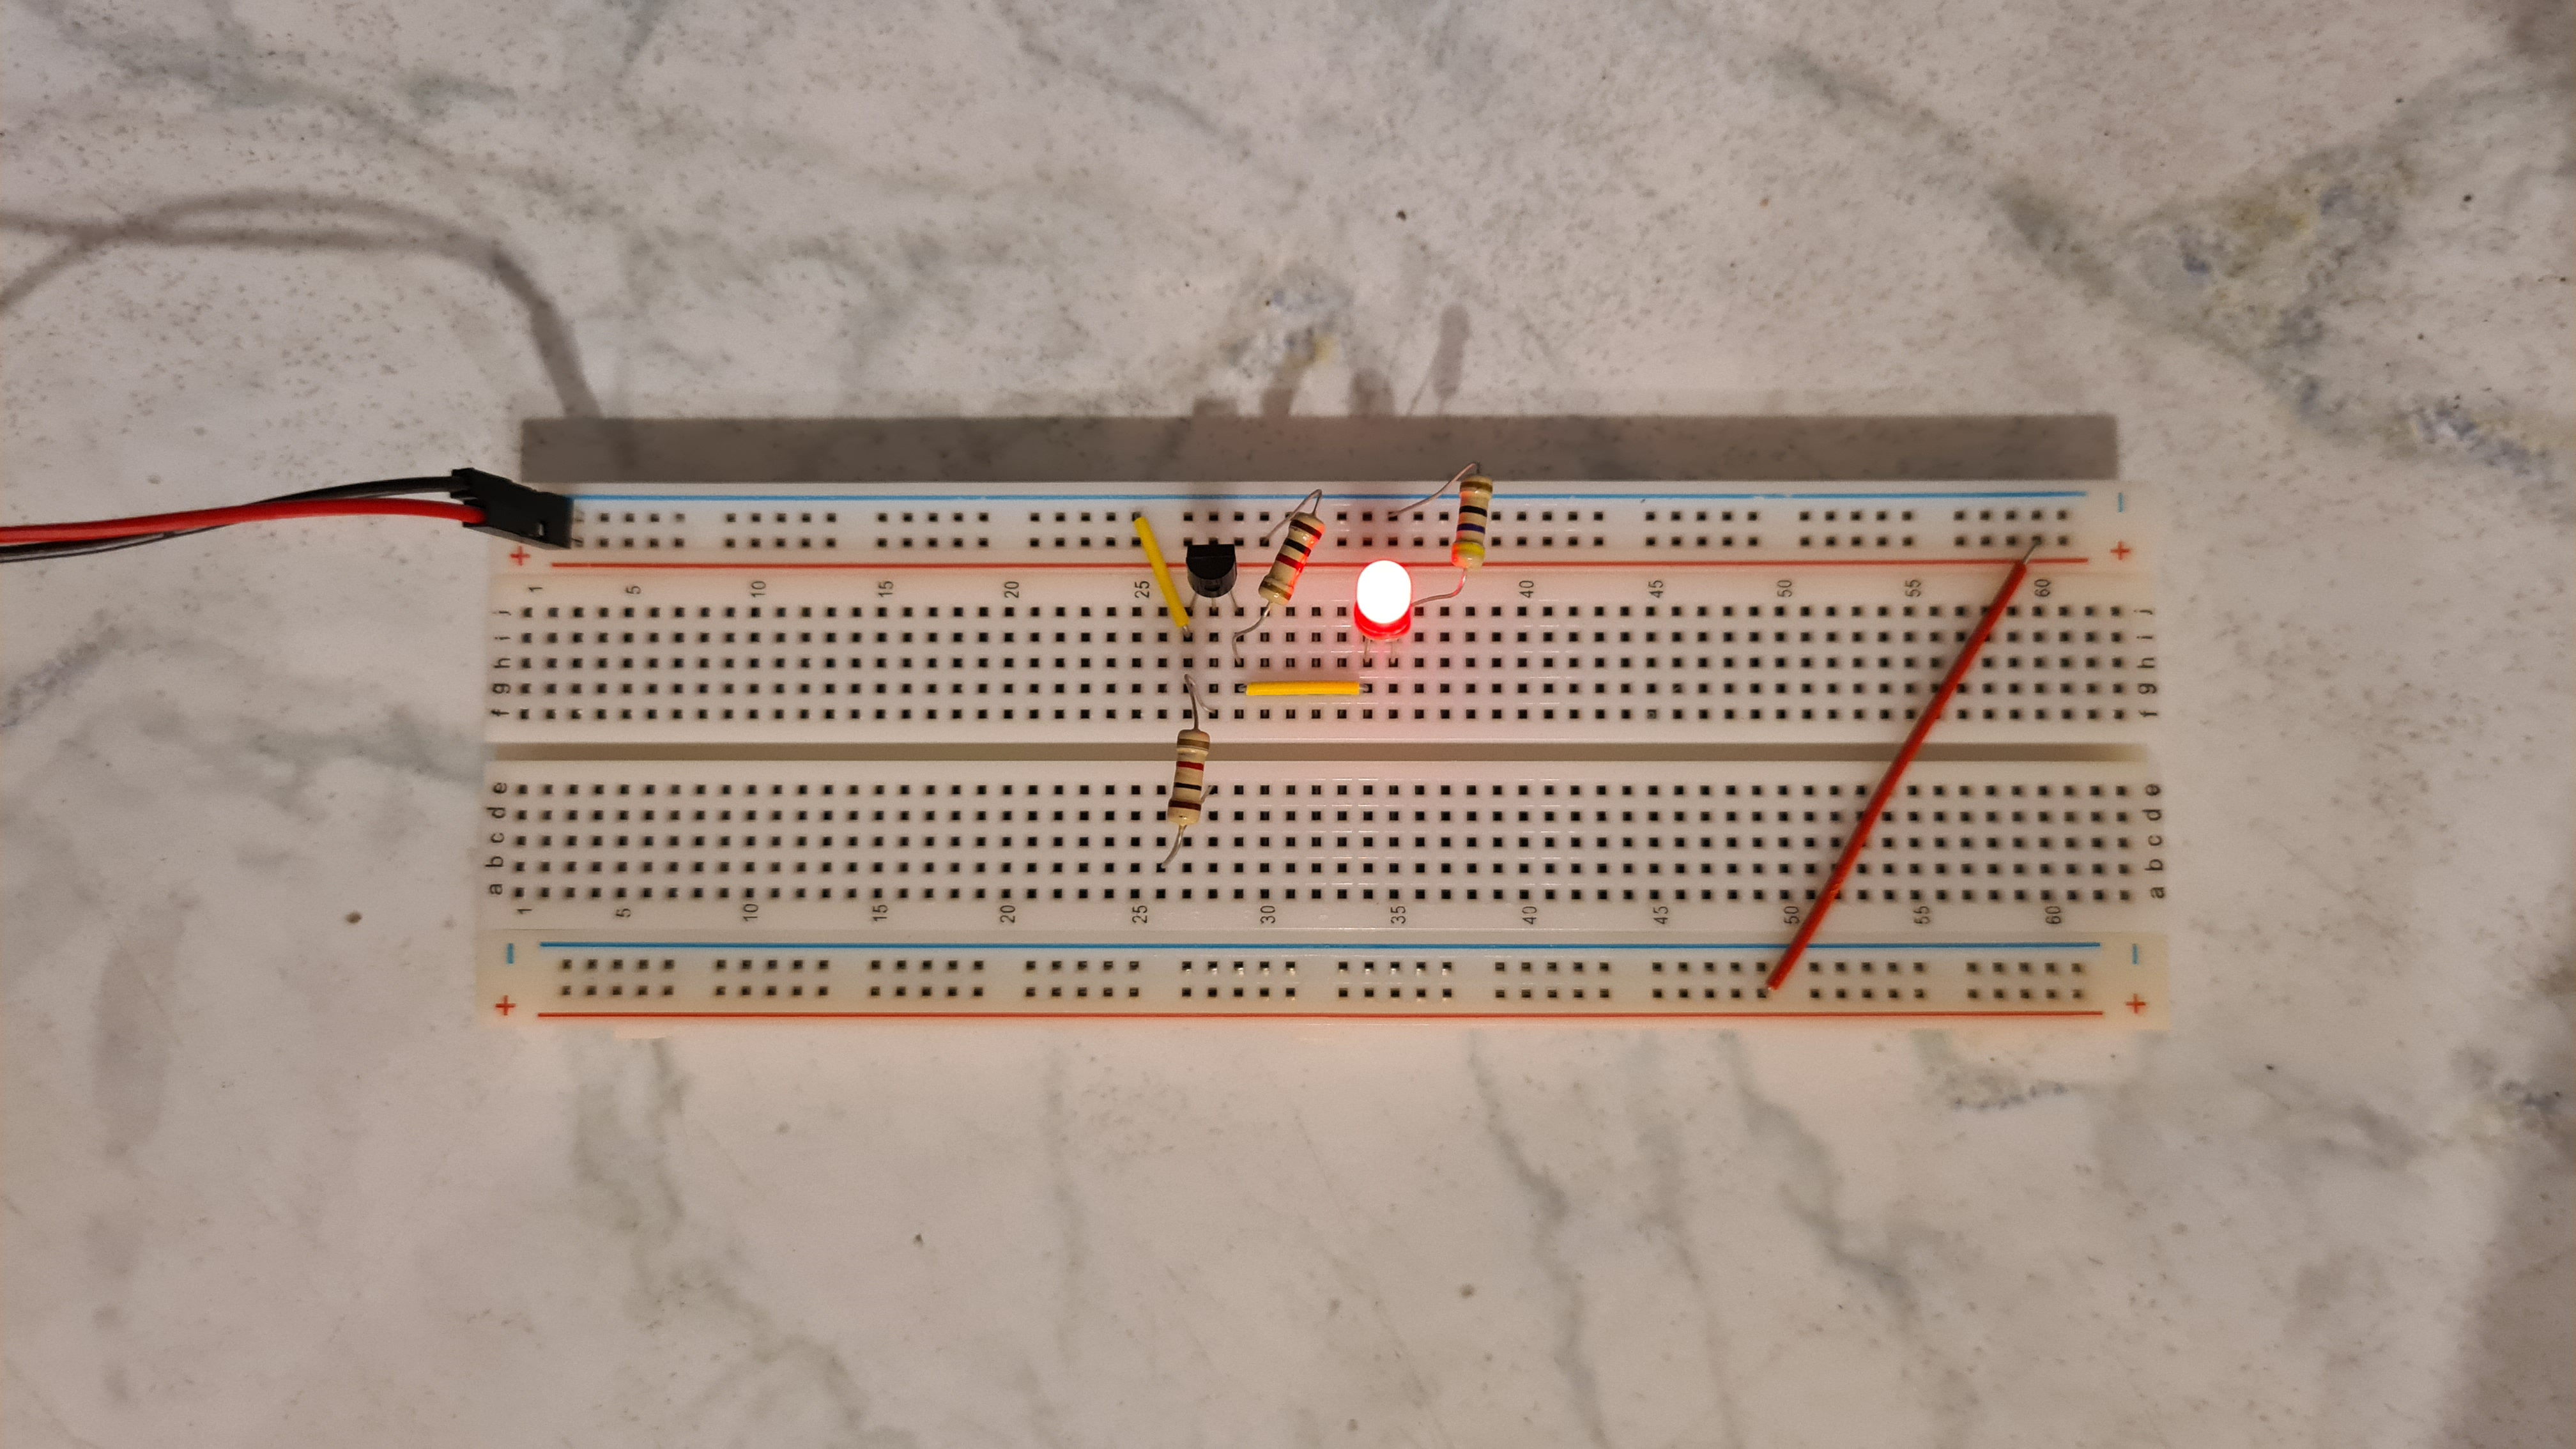
\includegraphics[height=4cm, keepaspectratio]{./Fotos/NICHT-0.jpg}
	\end{minipage}%
	\begin{minipage}{.5\textwidth}
		\centering
		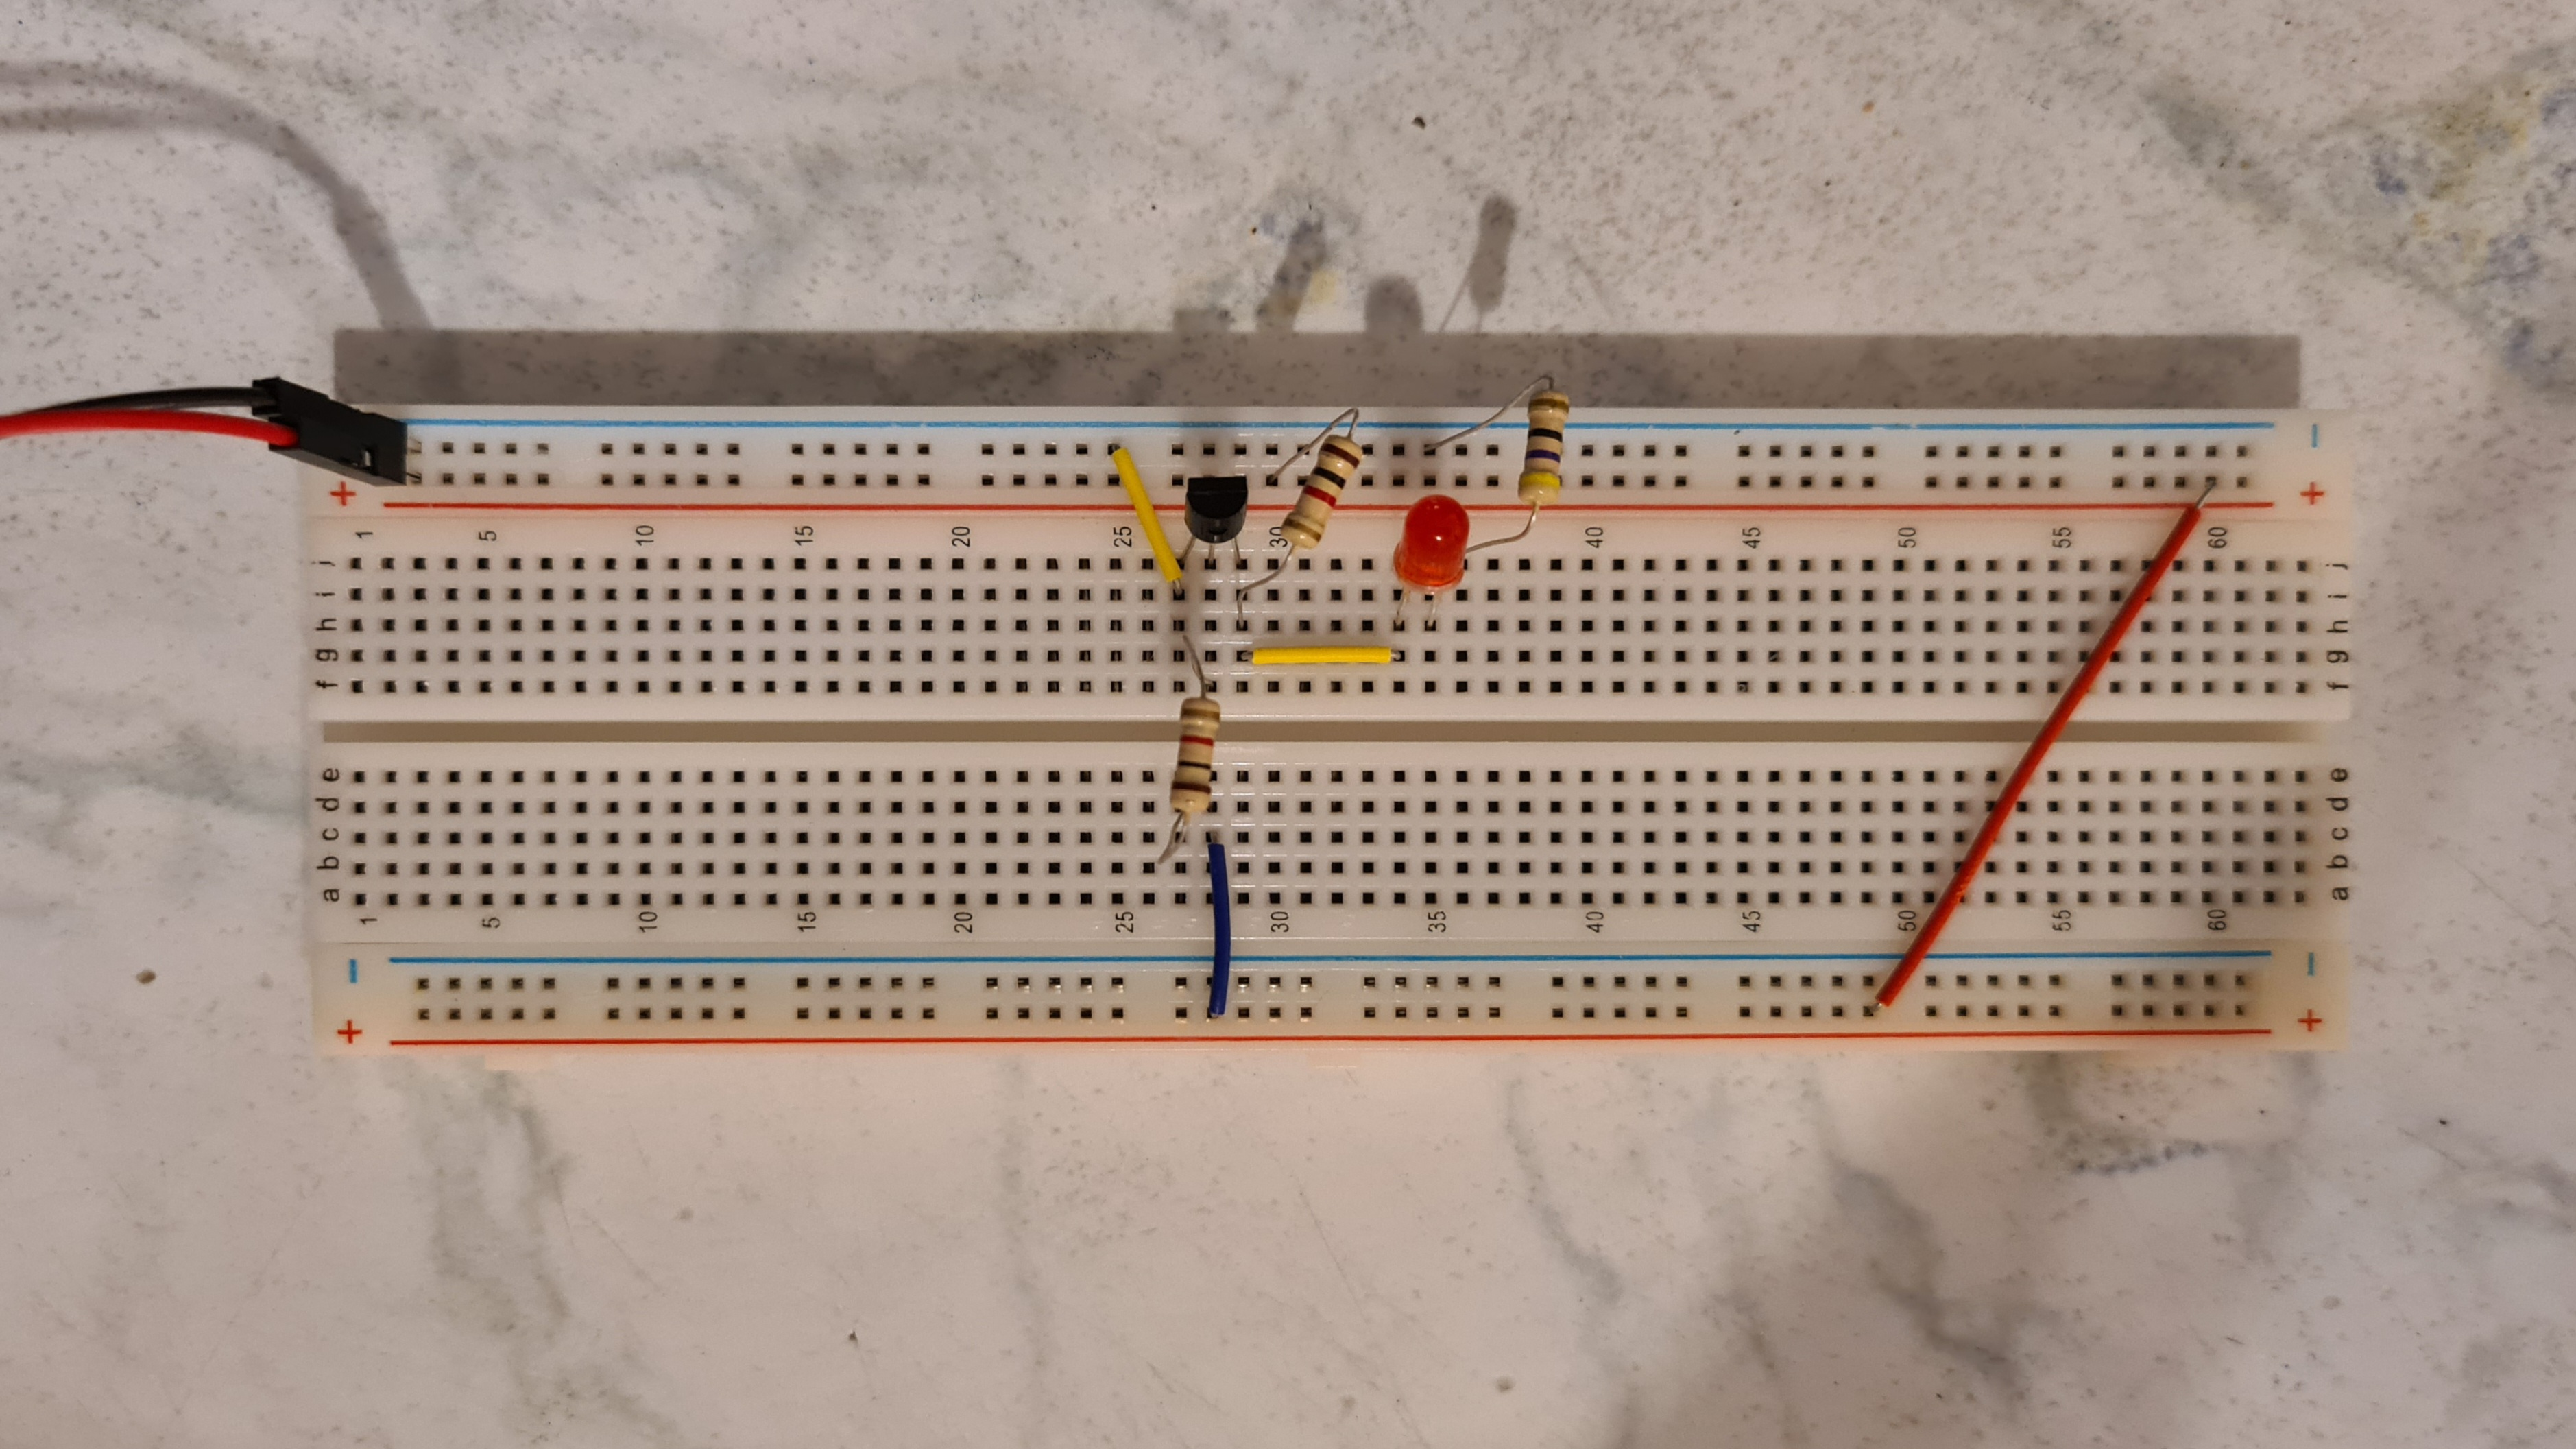
\includegraphics[height=4cm, keepaspectratio]{./Fotos/NICHT-1.jpg}
	\end{minipage}
	\caption{Praktischer Aufbau des NICHT-Gatters in allen möglichen Zuständen.}
\end{figure}
\newpage

\subsection{NAND-Gatter}
\begin{figure}[h]
	\centering
	\hspace{1cm}
	\begin{tabular}{|c|c|c|}
		\hline
		\textbf{A} & \textbf{B} & \textbf{Out} \\
		\hline
		0 & 0 & 1 \\
		1 & 0 & 1 \\
		0 & 1 & 1 \\
		1 & 1 & 0 \\
		\hline
	\end{tabular}
	\caption{Wahrheitstabelle für das logische NAND-Gatter}
\end{figure}
Wie in der Wahrheitstabelle zu erkennen, liegt Out auf HIGH, solange nicht A und B auf HIGH gesetzt sind. Das Verhalten dieses Gatters ist also gegenteilig zu dem des UND-Gatters. Der Name \gqq{NAND} setzt sich aus \gqq{NOT} und \gqq{AND} zusammen. Für das gewünschte Verhalten muss die Ausgabe eines UND-Gatters als Eingabe für ein NICHT-Gatter genutzt werden.\\
\begin{figure}[h!]
	\centering
	\begin{circuitikz}
		\draw (0, 0) node[npn](T1){$T_1$};
		\draw (0, -2) node[npn](T2){$T_2$};
		
		\draw (T1.B) to[R, l=$R_1$, a=\SI{2}{k\ohm}] ++(-2, 0) to[short, -o] ++(-.5, 0) node[left]{A};
		\draw (T2.B) to[R, l=$R_2$, a=\SI{2}{k\ohm}] ++(-2, 0) to[short, -o] ++(-.5, 0) node[left]{B};
		
		\draw (T1.C) to[short, -o] ++(0, 1) node[above]{$VCC$};
		\draw (T1.E) to[short] (T2.C);
		
		\draw (T2.E) to[R, l=$R_3$, a=\SI{330}{\ohm}] ++(0, -3) node[ground](GND){};
		
		\draw (5, -3) node[npn](T3){$T_3$};
		
		\draw (0, -3) to[short, *-] ++(1, 0) to[R, l=$R_4$, a=\SI{1}{k\ohm}] (T3.B);
		\draw (T3.E) to[short] ++(0, -1) node[ground](GND){};
		\draw (T3.C) to[short] ++(0, 1) to[R, l=$R_5$, a=\SI{1}{k\ohm}, -o] ++(0, 2) node[above]{$VCC$};
		
		\draw (5, -2) to[short, *-o] ++(2, 0) node[right]{Out};
		
		\draw[gray, very thick, densely dashed] (-3, 3) -- (6.5, 3) -- (6.5, -8) -- (-3, -8) -- cycle;
		\draw[lightgray, very thick, densely dashed] (-2.75, 2.75) -- (1.25, 2.75) -- (1.25, -6.75) -- (-2.75, -6.75) -- cycle;
		\draw[lightgray, very thick, densely dashed] (1.5, 2.75) -- (6.25, 2.75) -- (6.25, -6.75) -- (1.5, -6.75) -- cycle;
	
		\draw (6.5, -8) node[above right, gray]{NAND-Gatter};
		\draw (-.75, -6.75) node[below, gray]{UND-Gatter};
		\draw (3.875, -6.75) node[below, gray]{NICHT-Gatter};
	\end{circuitikz}
	\caption{Schaltplan für die logische NAND-Schaltung mithilfe von npn-Transistoren. Zusammengesetzt aus NICHT- und UND-Gatter}
\end{figure}\\
